% Khung Bài tập lớn – biên dịch bằng XeLaTeX, chạy 2 lần (latexmk -xelatex main.tex)
\RequirePackage{fix-cm}% font toán có đủ cỡ 13 pt, hết cảnh báo Size substitutions
\documentclass[a4paper]{report}
\usepackage{baocao}
\usepackage{amssymb}% \mathbb
\usepackage{rotating}% hình xoay ngang (sidewaysfigure)
\landscapepage{fig:landscape}% trang ngang: không Header, vẫn có Footer
\IfFileExists{dsfont.sty}{\usepackage{dsfont}\newcommand\ind{\mathds{1}}}{\newcommand\ind{\mathbb{1}}}% hàm chỉ thị
\def\UrlBreaks{\do\/\do\-\do\.}\Urlmuskip=0mu plus 2mu% cho phép URL xuống dòng
\usepackage{array,longtable}% bảng dài, cột tự xuống dòng
% ===== Thông tin trang bìa (sửa ở đây) =====
\khoa{Khoa Điện - Điện tử}% TODO: đúng khoa của bạn
\bomon{}% để trống nếu không cần dòng Bộ môn
\tenbaocao{Báo cáo bài tập lớn}
\monhoc{Máy học cơ bản và ứng dụng}
\detai{Dự đoán tái nhập viện của bệnh nhân đái tháo đường bằng các mô hình học máy}
\nhomlop{Tổ 10 - Nhóm L01}
\gvhd{PhD. Võ Tuấn Kiệt}
\thongtinsv{%
  Hồ Bá Chiến & 2310346 \\ \hline
  Trịnh Hoàng Dũng & 2310575 \\ \hline
  Phạm Lê Minh Sơn & 2312977 \\ \hline}
\tacgia{Tổ 10 - Nhóm L01}% Header trang lẻ


\begin{document}

\taobiatruoc% Bìa 1 + Bìa 2

\phantruoc
\tableofcontents
\chapter*{Từ viết tắt và ý nghĩa}
\addcontentsline{toc}{chapter}{\mdseries Từ viết tắt và ý nghĩa}
\begin{tuviettat}
  \item[AUC] Area Under the Curve – diện tích dưới đường cong ROC
  \item[DT] Decision Tree – cây quyết định
  \item[ICD-9] International Classification of Diseases, 9th revision – Phân loại quốc tế bệnh tật, bản sửa đổi lần 9
  \item[k-NN] k-nearest neighbors – k láng giềng gần nhất
  \item[LR] Logistic Regression – hồi quy logistic
  \item[MDI] Mean Decrease in Impurity – độ giảm độ không thuần khiết trung bình
  \item[MLP] Multi-Layer Perceptron – mạng perceptron nhiều lớp
  \item[OOB] Out-of-bag – mẫu ngoài túi
  \item[PCA] Principal Component Analysis – phân tích thành phần chính
  \item[ReLU] Rectified Linear Unit – hàm kích hoạt tuyến tính chỉnh lưu
  \item[RF] Random Forest – rừng ngẫu nhiên
  \item[ROC] Receiver Operating Characteristic – đường cong đặc trưng hoạt động của bộ thu
  \item[SVM] Support Vector Machine – máy vectơ hỗ trợ
\end{tuviettat}

\chapter*{Kí hiệu toán học}
\addcontentsline{toc}{chapter}{\mdseries Kí hiệu toán học}
\begin{tuviettat}
  \item[{$\ind[\cdot]$}] Hàm chỉ thị: bằng 1 nếu điều kiện đúng, ngược lại bằng 0
  \item[$x,\ x_i$] Vectơ đặc trưng của một mẫu; của mẫu thứ $i$
  \item[$y_i,\ \hat{y}$] Nhãn thật của mẫu thứ $i$; nhãn dự đoán
  \item[$n,\ N$] Số mẫu huấn luyện
  \item[$d$] Số chiều (số đặc trưng) của dữ liệu
  \item[$C$] Số lớp của nhãn
  \item[$c_k,\ K$] Loại thứ $k$ của một biến phân loại; số loại của biến
  \item[$\lambda_j$] Trị riêng thứ $j$ của ma trận hiệp phương sai (PCA)
  \item[$m,\ \tau$] Số thành phần chính giữ lại; ngưỡng phương sai tích lũy
  \item[$N_k(x)$] Tập $k$ láng giềng gần nhất của $x$
  \item[$d(x,x_i)$] Khoảng cách giữa $x$ và $x_i$
  \item[$w_i$] Trọng số của láng giềng (k-NN) hoặc của mô hình thứ $i$ (ensemble)
  \item[$W,\ b$] Ma trận trọng số và vectơ bias
  \item[$z,\ h^{(l)}$] Giá trị trước kích hoạt; đầu ra của lớp ẩn thứ $l$
  \item[$\lambda,\ \alpha$] Hệ số điều chuẩn L2
  \item[$\lVert\cdot\rVert_F$] Chuẩn Frobenius
  \item[$p_c$] Tỉ lệ mẫu thuộc lớp $c$ trong nút
  \item[$S,\ S_L,\ S_R$] Tập mẫu tại nút; tập con trái, phải sau khi chia
  \item[$B,\ T_b$] Số cây trong RF; cây thứ $b$
  \item[$M$] Số mô hình trong ensemble
  \item[$\mathcal{L}$] Hàm mất mát
\end{tuviettat}

\cleardoublepage\addcontentsline{toc}{chapter}{\mdseries Danh mục bảng biểu}
\listoftables
\cleardoublepage\addcontentsline{toc}{chapter}{\mdseries Danh mục hình}
\listoffigures

\phanchinh
% ======================================================================
\chuong{Đặt vấn đề và dữ liệu}

\section{ĐẶT VẤN ĐỀ VÀ MỤC TIÊU BÀI TOÁN}

\subsection{Đặt vấn đề}

Đái tháo đường là bệnh mạn tính cần theo dõi và điều trị liên tục. Sau khi xuất viện, nhiều bệnh nhân phải nhập viện lại vì điều trị chưa ổn định, biến chứng hoặc thiếu chăm sóc sau xuất viện. Tái nhập viện trong vòng 30 ngày làm tăng chi phí y tế, gây quá tải cho bệnh viện và thường được dùng như một chỉ báo chất lượng chăm sóc. Nếu nhận diện được nhóm nguy cơ cao ngay lúc xuất viện, bệnh viện có thể ưu tiên nguồn lực theo dõi, tái khám và can thiệp cho nhóm này.

Báo cáo dùng bộ dữ liệu \textit{Diabetes 130-US hospitals for years 1999–2008} (UCI Machine Learning Repository): 101.766 lượt nhập viện của bệnh nhân đái tháo đường (71.518 bệnh nhân) tại 130 bệnh viện Hoa Kỳ, gồm 50 thuộc tính (nhân khẩu học, thông tin nhập viện, xét nghiệm, chẩn đoán, thuốc điều trị và nhãn \texttt{readmitted}). Dữ liệu có nhiều giá trị khuyết, nhiều biến phân loại bậc cao (mã chẩn đoán theo International Classification of Diseases, bản sửa đổi lần 9, viết tắt là ICD-9) và nhãn imbalanced.

\subsection{Phát biểu bài toán}

Cho vector feature \textbf{x} của một lượt nhập viện, dự đoán nhãn \texttt{readmitted} $\in$ \{\texttt{<30}, \texttt{>30}, \texttt{NO}\}:

\begin{itemize}
  \item \textbf{Đa lớp:} \texttt{<30} (tái nhập viện trong 30 ngày), \texttt{>30} (sau 30 ngày), \texttt{NO} (không tái nhập viện).
  \item \textbf{Nhị phân:} \texttt{Readmitted} (\texttt{<30} hoặc \texttt{>30}) so với \texttt{Not readmitted} (\texttt{NO}).
\end{itemize}

Mục tiêu trọng tâm là phát hiện sớm các ca tái nhập viện trong 30 ngày.

\subsection{Mục tiêu}

\begin{itemize}
  \item Khảo sát dữ liệu gốc và tiền xử lý: bỏ thuộc tính định danh, xử lý giá trị khuyết, mã hóa biến phân loại.
  \item Xây dựng và so sánh các mô hình học máy cho bài toán dự đoán tái nhập viện.
  \item Đánh giá bằng các độ đo phù hợp với dữ liệu imbalanced.
  \item Phân tích các yếu tố liên quan đến nguy cơ tái nhập viện.
\end{itemize}

\subsection{Loại bỏ thuộc tính định danh}

Ba thuộc tính sau không mang ý nghĩa dự đoán nên bị loại (bảng~\ref{tb:dinhdanh}):

{\small\setstretch{1.0}\renewcommand\arraystretch{1.1}\setlength\tabcolsep{3pt}
\begin{longtable}{|>{\raggedright\arraybackslash}p{74.31pt}|>{\centering\arraybackslash}p{103.17pt}|>{\raggedright\arraybackslash}p{257.16pt}|}
\caption{Các thuộc tính định danh bị loại bỏ}\label{tb:dinhdanh}\\
\hline
\textbf{Thuộc tính} & \textbf{Số giá trị khác nhau} & \textbf{Lý do loại bỏ} \\ \hline\endfirsthead
\caption[]{Các thuộc tính định danh bị loại bỏ (tiếp theo)}\\
\hline
\textbf{Thuộc tính} & \textbf{Số giá trị khác nhau} & \textbf{Lý do loại bỏ} \\ \hline\endhead
\texttt{encounter\_\allowbreak{}id} & 101.766 & Mã lượt nhập viện, duy nhất cho mỗi dòng; chỉ là khóa, không khái quát được. \\ \hline
\texttt{patient\_\allowbreak{}nbr} & 71.518 & Mã bệnh nhân; giữ lại dễ khiến mô hình ghi nhớ bệnh nhân và data leakage giữa tập train và test. \\ \hline
\texttt{payer\_\allowbreak{}code} & 17 & Mã bên thanh toán; khuyết 39,56\% và là thông tin hành chính, ít liên quan lâm sàng. \\ \hline
\end{longtable}
}

Kết quả: 101.766 × 50 $\rightarrow$ \textbf{101.766 × 47}.

\subsection{Thống kê khuyết và lọc thuộc tính khuyết > 50\%}

Ngưỡng loại bỏ là 50\%; tỉ lệ khuyết và cách xử lý nêu ở bảng~\ref{tb:khuyet}.

{\small\setstretch{1.0}\renewcommand\arraystretch{1.1}\setlength\tabcolsep{3pt}
\begin{longtable}{|>{\raggedright\arraybackslash}p{144.88pt}|>{\centering\arraybackslash}p{144.88pt}|>{\raggedright\arraybackslash}p{144.88pt}|}
\caption{Tỉ lệ khuyết của các thuộc tính và cách xử lý}\label{tb:khuyet}\\
\hline
\textbf{Thuộc tính} & \textbf{Tỉ lệ khuyết} & \textbf{Xử lý} \\ \hline\endfirsthead
\caption[]{Tỉ lệ khuyết của các thuộc tính và cách xử lý (tiếp theo)}\\
\hline
\textbf{Thuộc tính} & \textbf{Tỉ lệ khuyết} & \textbf{Xử lý} \\ \hline\endhead
\texttt{weight} & 96,86\% & \textbf{Loại bỏ} \\ \hline
\texttt{max\_\allowbreak{}glu\_\allowbreak{}serum} & 94,75\% & \textbf{Loại bỏ} \\ \hline
\texttt{A1Cresult} & 83,28\% & \textbf{Loại bỏ} \\ \hline
\texttt{medical\_\allowbreak{}specialty} & 49,08\% & Giữ (sát ngưỡng, xử lý ở bước sau) \\ \hline
\texttt{race}, \texttt{diag\_\allowbreak{}3}, \texttt{diag\_\allowbreak{}2}, \texttt{diag\_\allowbreak{}1} & 2,23\% / 1,40\% / 0,35\% / 0,02\% & Giữ (khuyết ít) \\ \hline
\end{longtable}
}

Kết quả: 101.766 × 47 $\rightarrow$ \textbf{101.766 × 44}.

\section{KHẢO SÁT CÁC NGHIÊN CỨU LIÊN QUAN}

Các nghiên cứu học máy về đái tháo đường có thể chia thành hai hướng: (i) chẩn đoán/dự đoán mắc bệnh trên dữ liệu nhỏ, và (ii) dự đoán biến cố lâm sàng như nhập viện hay tái nhập viện trên dữ liệu bệnh án điện tử lớn. Bài toán của báo cáo này thuộc hướng thứ hai.

\begin{itemize}
  \item \textbf{Dữ liệu nhỏ, dự đoán mắc bệnh.} Nhiều công trình dùng bộ Pima Indians Diabetes (PIDD, khoảng 700 bệnh nhân). Khanam và Foo (2021) \cite{tl1} so sánh các thuật toán học máy trên bộ dữ liệu này; Dutta và cộng sự (2018) \cite{tl4} dùng Logistic Regression (LR), Support Vector Machine (SVM) và Random Forest (RF), đạt accuracy khoảng 84\% và phân tích feature importance; Sisodia và Sisodia (2018) \cite{tl5} dùng Naive Bayes và các bộ phân loại khác. Một số báo cáo đạt tới 90\% (Maniruzzaman và cộng sự, 2018 \cite{tl2}, nhấn mạnh vai trò của giá trị khuyết và ngoại lai). Hạn chế chung là kích thước mẫu nhỏ, dễ overfitting, nên accuracy cao khó khái quát hóa.

  \item \textbf{Dữ liệu bệnh án lớn.} Brisimi và cộng sự (2019) \cite{tl3} dùng dữ liệu hồ sơ sức khỏe điện tử khoảng 40.000 bệnh nhân vùng Boston, kết hợp phân cụm trước khi phân loại, đạt accuracy khoảng 89\%. Hasan và cộng sự (2020) \cite{tl6} đề xuất ensemble k-nearest neighbors (k-NN), Decision Tree (DT), Random Forest, Naive Bayes và Multi-Layer Perceptron (MLP), lấy weighted average theo diện tích dưới đường cong ROC (Receiver Operating Characteristic), viết tắt là AUC (Area Under the Curve), của từng mô hình.

  \item \textbf{Dữ liệu tái nhập viện.} Strack và cộng sự (2014) \cite{tl7} công bố bộ dữ liệu 130 bệnh viện Hoa Kỳ (1999–2008) và phân tích tác động của xét nghiệm HbA1c lên tỉ lệ tái nhập viện – đây chính là nguồn dữ liệu của báo cáo. Wang (Stanford CS229) \cite{tl8} áp dụng trên bộ này k-NN, Logistic Regression, Decision Tree, Random Forest, neural network và mô hình ensemble, với Principal Component Analysis (PCA) để giảm chiều sau mã hóa one-hot (từ khoảng 2.500 chiều xuống 60). Kết quả: accuracy khoảng 38–40\% cho bài toán 3 lớp và khoảng 60–63\% cho bài toán nhị phân; neural network tốt nhất nhưng chỉ nhỉnh hơn k-NN không đáng kể. Tác giả chỉ ra các điểm yếu: class imbalance khiến mô hình thiên về dự đoán “không tái nhập viện”, accuracy trung bình theo lớp thấp, PCA làm mất khả năng diễn giải, và chưa thử huấn luyện trên dữ liệu cân bằng.

  \item \textbf{Khoảng trống và hướng của báo cáo.} Từ khảo sát trên, báo cáo này (1) xây dựng cả nhãn đa lớp (\texttt{<30}, \texttt{>30}, \texttt{NO}) và nhãn nhị phân (\texttt{Readmitted} so với \texttt{Not readmitted}), trong đó nhóm \texttt{<30} được giữ riêng để phục vụ mục tiêu phát hiện sớm tái nhập viện trong 30 ngày, (2) tính đến class imbalance và đánh giá bằng macro-F1, F1 từng lớp và AUC thay vì chỉ Accuracy, (3) dùng PCA 60 thành phần cho các mô hình dựa trên khoảng cách và tuyến tính, đồng thời nêu rõ giới hạn của PCA (mất khả năng diễn giải, phương sai giải thích thấp khi One-Hot nhiều mã ICD-9 hiếm) và dùng mô hình cây/rừng cùng phân tích feature importance để bổ sung khả năng diễn giải.
\end{itemize}

\section{MÔ TẢ CHI TIẾT TẬP DỮ LIỆU LÂM SÀNG GỐC}

\subsection{Nguồn dữ liệu}

Bộ dữ liệu (nguồn, quy mô, số bệnh nhân: xem 1.1.1) là file \texttt{diabetic\_\allowbreak{}data.csv}, mỗi dòng ứng với một lượt nhập viện; một bệnh nhân có thể xuất hiện ở nhiều dòng. Giá trị khuyết được mã hóa bằng ký tự \texttt{?} (không phải \texttt{NaN} chuẩn), cần khai báo khi đọc dữ liệu (\texttt{na\_\allowbreak{}values="?"}).

Danh sách đầy đủ 50 cột (lấy trực tiếp khi đọc \texttt{diabetic\_\allowbreak{}data.csv}):

{\scriptsize
\begin{verbatim}
encounter_id, patient_nbr, race, gender, age, weight, admission_type_id,
discharge_disposition_id, admission_source_id, time_in_hospital, payer_code,
medical_specialty, num_lab_procedures, num_procedures, num_medications,
number_outpatient, number_emergency, number_inpatient, diag_1, diag_2, diag_3,
number_diagnoses, max_glu_serum, A1Cresult, metformin, repaglinide, nateglinide,
chlorpropamide, glimepiride, acetohexamide, glipizide, glyburide, tolbutamide,
pioglitazone, rosiglitazone, acarbose, miglitol, troglitazone, tolazamide,
examide, citoglipton, insulin, glyburide-metformin, glipizide-metformin,
glimepiride-pioglitazone, metformin-rosiglitazone, metformin-pioglitazone,
change, diabetesMed, readmitted
\end{verbatim}
}

Ví dụ 2 dòng dữ liệu đầu, trình bày ở bảng~\ref{tb:vidu} (rút gọn để minh họa định dạng, giá trị khuyết hiển thị là \texttt{?}):

{\scriptsize\setstretch{1.0}\renewcommand\arraystretch{1.1}\setlength\tabcolsep{1.5pt}
\begin{longtable}{|>{\raggedright\arraybackslash}p{36.62pt}|>{\raggedright\arraybackslash}p{26.34pt}|>{\centering\arraybackslash}p{26.99pt}|>{\centering\arraybackslash}p{25.56pt}|>{\raggedright\arraybackslash}p{25.56pt}|>{\raggedright\arraybackslash}p{25.56pt}|>{\raggedright\arraybackslash}p{26.70pt}|>{\raggedright\arraybackslash}p{48.10pt}|>{\raggedright\arraybackslash}p{41.83pt}|}
\caption{Hai dòng dữ liệu đầu tiên (rút gọn)}\label{tb:vidu}\\
\hline
\textbf{race} & \textbf{gender} & \textbf{age} & \textbf{diag\_\allowbreak{}1} & \textbf{diag\_\allowbreak{}2} & \textbf{diag\_\allowbreak{}3} & \textbf{change} & \textbf{diabetesMed} & \textbf{readmitted} \\ \hline\endfirsthead
\caption[]{Hai dòng dữ liệu đầu tiên (rút gọn) (tiếp theo)}\\
\hline
\textbf{race} & \textbf{gender} & \textbf{age} & \textbf{diag\_\allowbreak{}1} & \textbf{diag\_\allowbreak{}2} & \textbf{diag\_\allowbreak{}3} & \textbf{change} & \textbf{diabetesMed} & \textbf{readmitted} \\ \hline\endhead
Caucasian & Female & [0-10) & 250.83 & ? & ? & No & No & NO \\ \hline
Caucasian & Female & [10-20) & 276 & 250.01 & 255 & Ch & Yes & >30 \\ \hline
\end{longtable}
}

\subsection{Các nhóm thuộc tính (50 cột)}

Các nhóm thuộc tính được tóm tắt ở bảng~\ref{tb:nhom}:

{\small\setstretch{1.0}\renewcommand\arraystretch{1.1}\setlength\tabcolsep{3pt}
\begin{longtable}{|>{\raggedright\arraybackslash}p{118.46pt}|>{\raggedright\arraybackslash}p{158.09pt}|>{\raggedright\arraybackslash}p{158.09pt}|}
\caption{Các nhóm thuộc tính của bộ dữ liệu}\label{tb:nhom}\\
\hline
\textbf{Nhóm} & \textbf{Thuộc tính} & \textbf{Ghi chú} \\ \hline\endfirsthead
\caption[]{Các nhóm thuộc tính của bộ dữ liệu (tiếp theo)}\\
\hline
\textbf{Nhóm} & \textbf{Thuộc tính} & \textbf{Ghi chú} \\ \hline\endhead
Định danh & \texttt{encounter\_\allowbreak{}id}, \texttt{patient\_\allowbreak{}nbr}, \texttt{payer\_\allowbreak{}code} & Không mang ý nghĩa dự đoán / có nguy cơ data leakage \\ \hline
Nhân khẩu học & \texttt{race} (5 nhóm), \texttt{gender} (3 giá trị: \texttt{Female} 54.708, \texttt{Male} 47.055, \texttt{Unknown/\allowbreak{}Invalid} 3 dòng), \texttt{age} (10 khoảng 10 tuổi, đông nhất \texttt{[70-80)} với 26.068 dòng), \texttt{weight} (khoảng cân nặng, ví dụ \texttt{[75-100)}) & \texttt{weight} khuyết $\approx$ 96,86\% \\ \hline
Thông tin lượt nhập viện & \texttt{admission\_\allowbreak{}type\_\allowbreak{}id} (8 mã), \texttt{discharge\_\allowbreak{}disposition\_\allowbreak{}id} (26 mã), \texttt{admission\_\allowbreak{}source\_\allowbreak{}id} (17 mã), \texttt{time\_\allowbreak{}in\_\allowbreak{}hospital} (1–14 ngày), \texttt{medical\_\allowbreak{}specialty} (72 giá trị) & Ba cột \texttt{*\_\allowbreak{}id} là mã phân loại, không phải số thứ tự có quan hệ thứ bậc \\ \hline
Xét nghiệm và thủ thuật & \texttt{num\_\allowbreak{}lab\_\allowbreak{}procedures}, \texttt{num\_\allowbreak{}procedures}, \texttt{num\_\allowbreak{}medications}, \texttt{number\_\allowbreak{}diagnoses} (1–16), \texttt{max\_\allowbreak{}glu\_\allowbreak{}serum} (\texttt{Norm}, \texttt{>200}, \texttt{>300}), \texttt{A1Cresult} (\texttt{Norm}, \texttt{>7}, \texttt{>8}) & \texttt{max\_\allowbreak{}glu\_\allowbreak{}serum} khuyết $\approx$ 94,75\%, \texttt{A1Cresult} khuyết $\approx$ 83,28\% (khuyết nghĩa là không làm xét nghiệm) \\ \hline
Tiền sử sử dụng dịch vụ & \texttt{number\_\allowbreak{}outpatient}, \texttt{number\_\allowbreak{}emergency}, \texttt{number\_\allowbreak{}inpatient} & Số lần trong năm trước lượt nhập viện hiện tại (tối đa lần lượt 42, 76, 21) \\ \hline
Chẩn đoán & \texttt{diag\_\allowbreak{}1}, \texttt{diag\_\allowbreak{}2}, \texttt{diag\_\allowbreak{}3} & Mã ICD-9, số giá trị khác nhau rất lớn: 716 (\texttt{diag\_\allowbreak{}1}), 748 (\texttt{diag\_\allowbreak{}2}), 789 (\texttt{diag\_\allowbreak{}3}) \\ \hline
Thuốc (23 cột) & \texttt{metformin}, \texttt{insulin}, \texttt{glipizide}, \texttt{glyburide}, \texttt{repaglinide}, \texttt{nateglinide}, \texttt{chlorpropamide}, \texttt{glimepiride}, \texttt{acetohexamide}, \texttt{tolbutamide}, \texttt{pioglitazone}, \texttt{rosiglitazone}, \texttt{acarbose}, \texttt{miglitol}, \texttt{troglitazone}, \texttt{tolazamide}, \texttt{examide}, \texttt{citoglipton}, \texttt{glyburide-\allowbreak{}metformin}, \texttt{glipizide-\allowbreak{}metformin}, \texttt{glimepiride-\allowbreak{}pioglitazone}, \texttt{metformin-\allowbreak{}rosiglitazone}, \texttt{metformin-\allowbreak{}pioglitazone} & Tối đa 4 mức: \texttt{No}, \texttt{Steady}, \texttt{Up}, \texttt{Down}. Một số cột ít mức hơn: \texttt{examide}, \texttt{citoglipton} chỉ có \texttt{No}; \texttt{tolazamide} có 3 mức; \texttt{acetohexamide}, \texttt{tolbutamide}, \texttt{troglitazone}, \texttt{glipizide-\allowbreak{}metformin}, \texttt{glimepiride-\allowbreak{}pioglitazone}, \texttt{metformin-\allowbreak{}rosiglitazone}, \texttt{metformin-\allowbreak{}pioglitazone} có 2 mức \\ \hline
Tổng hợp điều trị & \texttt{change} (\texttt{Ch}/\texttt{No}), \texttt{diabetesMed} (\texttt{Yes}/\texttt{No}) & Có thay đổi thuốc / có dùng thuốc đái tháo đường trong lượt nhập viện \\ \hline
Nhãn & \texttt{readmitted} & \texttt{NO} 54.864 (53,9\%), \texttt{>30} 35.545 (34,9\%), \texttt{<30} 11.357 (11,2\%) \\ \hline
\end{longtable}
}

\subsection{Đặc điểm cần xử lý}

\begin{itemize}
  \item \textbf{Giá trị khuyết}: \texttt{weight}, \texttt{max\_\allowbreak{}glu\_\allowbreak{}serum}, \texttt{A1Cresult} khuyết trên 80\%, \texttt{medical\_\allowbreak{}specialty} gần 50\%, \texttt{payer\_\allowbreak{}code} gần 40\%; tỉ lệ khuyết đầy đủ ở bảng~\ref{tb:khuyet}, cách xử lý ở 1.1.4 và 1.1.5.
  \item \textbf{Thuộc tính hằng số hoặc gần hằng số}: \texttt{examide} và \texttt{citoglipton} chỉ nhận một giá trị duy nhất (\texttt{No}) trong toàn bộ dữ liệu nên không mang thông tin phân biệt; bảy cột thuốc khác chỉ có 2 mức (\texttt{acetohexamide}, \texttt{tolbutamide}, \texttt{troglitazone}, \texttt{glipizide-\allowbreak{}metformin}, \texttt{glimepiride-\allowbreak{}pioglitazone}, \texttt{metformin-\allowbreak{}rosiglitazone}, \texttt{metformin-\allowbreak{}pioglitazone}), hầu hết dòng đều là \texttt{No}. Sau One-Hot, \texttt{examide\_\allowbreak{}No} và \texttt{citoglipton\_\allowbreak{}No} toàn bằng 1 (phương sai 0) và bị bước 05 loại khỏi PCA (ngưỡng phương sai 1e-9), nên PCA chạy trên 2.394 trong 2.396 cột (xem 3.1.5).
  \item \textbf{Biến phân loại bậc cao}: mã chẩn đoán ICD-9 (\texttt{diag\_\allowbreak{}1/\allowbreak{}2/\allowbreak{}3}, 716 đến 789 giá trị), \texttt{medical\_\allowbreak{}specialty} (72 giá trị) và ba cột \texttt{*\_\allowbreak{}id} (\texttt{admission\_\allowbreak{}type\_\allowbreak{}id} 8 mã, \texttt{discharge\_\allowbreak{}disposition\_\allowbreak{}id} 26 mã, \texttt{admission\_\allowbreak{}source\_\allowbreak{}id} 17 mã) cần mã hóa phù hợp trước khi đưa vào mô hình.
  \item \textbf{Class imbalance}: lớp \texttt{<30} (tái nhập viện trong 30 ngày) chỉ chiếm khoảng 11,2\% (11.357 dòng) – cần độ đo đánh giá phù hợp (Recall, F1, ROC-AUC/PR-AUC) thay vì chỉ accuracy. Ở bài toán nhị phân hai lớp gần cân bằng (\texttt{y\_\allowbreak{}bin = 1} chiếm 46,19\% tập train).
  \item \textbf{Nhiều lượt nhập viện trên cùng một bệnh nhân}: 101.766 dòng nhưng chỉ có 71.518 bệnh nhân khác nhau $\rightarrow$ khi chia train/test cần nhóm theo \texttt{patient\_\allowbreak{}nbr} để một bệnh nhân không xuất hiện ở cả hai tập, tránh data leakage (làm ở bước 03).
\end{itemize}

\subsection{Xử lý dữ liệu: lọc dòng khuyết, tạo nhãn và chia train/test}

Lọc dòng khuyết < 2\%, tạo hai bộ nhãn \texttt{y\_\allowbreak{}multi}, \texttt{y\_\allowbreak{}bin} và chia train/test 80/20 theo bệnh nhân được trình bày ở 3.1.2 và 3.1.3.

\chuong{Cơ sở lý thuyết}

\section{MÃ HÓA ONE-HOT VÀ CƠ SỞ TOÁN HỌC PCA}

\subsection{Mã hóa One-Hot}

Các mô hình k-NN và Logistic Regression chỉ làm việc với số. Nếu mã hóa nhãn một biến phân loại thành 1, 2, 3, … thì mô hình hiểu nhầm có thứ tự và khoảng cách giữa các loại (ví dụ mã ICD-9 \texttt{250} “gần” \texttt{251} hơn \texttt{401}). One-Hot Encoding tránh điều này: biến $x$ có $K$ giá trị được thay bằng $K$ cột nhị phân

\begin{equation}
  e_k(x) = \ind[x = c_k],\quad k = 1,\dots,K,
\end{equation}

trong đó $x$ là biến phân loại, $c_k$ là giá trị thứ $k$ của $x$ và $\ind[\cdot]$ là hàm chỉ thị (bằng 1 nếu điều kiện đúng, ngược lại bằng 0); mỗi dòng có đúng một cột bằng 1. Khoảng cách giữa hai loại khác nhau luôn bằng $\sqrt{2}$, nên không loại nào “gần” loại nào.

Áp dụng trên tập train/test đã qua các bước 01–03 (tập train: 79.726 dòng, tập test: 20.518 dòng; mỗi tập 43 feature và 2 nhãn \texttt{y\_\allowbreak{}multi}, \texttt{y\_\allowbreak{}bin}).

\begin{itemize}
  \item \textbf{Biến được mã hóa (35):} 32 thuộc tính chữ (\texttt{race}, \texttt{gender}, \texttt{age}, \texttt{medical\_\allowbreak{}specialty}, 3 mã chẩn đoán ICD-9 \texttt{diag\_\allowbreak{}1..3}, các thuốc, \texttt{change}, \texttt{diabetesMed}, …) và 3 mã số thực chất là mã loại: \texttt{admission\_\allowbreak{}type\_\allowbreak{}id}, \texttt{discharge\_\allowbreak{}disposition\_\allowbreak{}id}, \texttt{admission\_\allowbreak{}source\_\allowbreak{}id}. Hai nhãn \texttt{y\_\allowbreak{}multi}, \texttt{y\_\allowbreak{}bin} được tách ra, không mã hóa.
  \item \textbf{Giá trị khuyết:} coi là một loại riêng \texttt{Missing} (khuyết có thể mang thông tin, ví dụ \texttt{medical\_\allowbreak{}specialty} không ghi). Sau bước 03, chỉ còn \texttt{race} và \texttt{medical\_\allowbreak{}specialty} có giá trị khuyết.
  \item \textbf{Biến số giữ nguyên (8):} \texttt{time\_\allowbreak{}in\_\allowbreak{}hospital}, \texttt{num\_\allowbreak{}lab\_\allowbreak{}procedures}, \texttt{num\_\allowbreak{}procedures}, \texttt{num\_\allowbreak{}medications}, \texttt{number\_\allowbreak{}outpatient}, \texttt{number\_\allowbreak{}emergency}, \texttt{number\_\allowbreak{}inpatient}, \texttt{number\_\allowbreak{}diagnoses}.
  \item \textbf{Fit trên train:} tập loại của mỗi biến chỉ được học từ tập train, rồi áp dụng sang test. Đặt \texttt{handle\_\allowbreak{}unknown="ignore"} để loại chỉ có ở test (ví dụ mã ICD-9 hiếm) được mã hóa thành toàn 0, tránh để thông tin của tập test lọt vào bước tiền xử lý.
  \item \textbf{Kết quả:} 8 biến số + 2.388 cột One-Hot = \textbf{2.396 cột} (train 79.726 × 2.396, test 20.518 × 2.396). \texttt{diag\_\allowbreak{}1}, \texttt{diag\_\allowbreak{}2}, \texttt{diag\_\allowbreak{}3} có lần lượt 697, 716, 761 cột, chiếm khoảng 91\% số cột One-Hot.
  \item \textbf{Lưu trữ:} ma trận rất thưa (mỗi dòng chỉ có 35 giá trị 1 trên 2.388 cột One-Hot), nên được lưu dạng ma trận thưa (sparse).
\end{itemize}

Kích thước 2.396 chiều, phần lớn là các mã ICD-9 hiếm, là lý do cần dimensionality reduction bằng PCA.

\subsection{Cơ sở toán học của PCA}

PCA tìm một phép chiếu tuyến tính sang không gian ít chiều sao cho giữ lại nhiều phương sai nhất. Cho ma trận dữ liệu $X \in \mathbb{R}^{n \times d}$, đã trừ trung bình từng cột ($\bar{X}$).

\begin{itemize}
  \item \textbf{Covariance matrix:} $\;C = \dfrac{1}{n-1}\bar{X}^{\top}\bar{X} \in \mathbb{R}^{d\times d}$.
  \item \textbf{Phân rã trị riêng:} $C v_j = \lambda_j v_j$ với $\lambda_1 \ge \lambda_2 \ge \dots \ge \lambda_d \ge 0$ và $v_j$ trực chuẩn. Principal component thứ $j$ là hướng $v_j$, phương sai dọc theo nó bằng $\lambda_j$.
  \item \textbf{Chọn $m$ thành phần:} $\;Z = \bar{X} V_m,\; V_m = [v_1,\dots,v_m]$, và chọn $m$ nhỏ nhất sao cho tỉ lệ phương sai giải thích
\end{itemize}

\begin{equation}
  \frac{\sum_{j=1}^{m}\lambda_j}{\sum_{j=1}^{d}\lambda_j} \ge \tau \quad(\text{ví dụ } \tau = 0{,}95).
\end{equation}

Trong đó $\tau$ là ngưỡng tỉ lệ phương sai giải thích tối thiểu, $m$ là số thành phần giữ lại, $d$ là số chiều ban đầu và $\lambda_j$ là trị riêng thứ $j$. PCA tương đương cực tiểu sai số tái tạo $\lVert \bar{X} - \bar{X}V_mV_m^{\top}\rVert_F^2$. Trong thực hành tính qua SVD $\bar{X} = U\Sigma V^{\top}$, khi đó $\lambda_j = \sigma_j^2/(n-1)$ và không cần tạo ra $C$.

\textbf{PCA trên correlation matrix.} Dữ liệu trộn cột số (ví dụ \texttt{num\_\allowbreak{}lab\_\allowbreak{}procedures} tới hơn 100) với cột nhị phân 0/1, nên nếu dùng covariance matrix thì cột số lấn át. Vì vậy ta scale từng cột về trung bình 0, độ lệch chuẩn 1 trước, tương đương phân rã correlation matrix $R = D^{-1/2} C D^{-1/2}$ với $D = \mathrm{diag}(C)$. Các cột có phương sai 0 trên train bị bỏ (không chia được cho độ lệch chuẩn).

\textbf{Tính trên ma trận thưa.} Trừ trung bình làm ma trận One-Hot mất tính thưa. Có thể tránh việc này: tính $C = \frac{1}{n}X^{\top}X - \mu\mu^{\top}$ trực tiếp từ $X$ thưa, và chiếu $Z = \big((X - \mathbf{1}\mu^{\top})\,D^{-1/2}\big)V_m = X\,(D^{-1/2}V_m) - \mathbf{1}\,(\mu^{\top}D^{-1/2}V_m)$, nên không bao giờ phải tạo ma trận dày cỡ $n \times d$. Trung bình $\mu$, độ lệch chuẩn và $V_m$ chỉ học từ train rồi áp dụng sang test.

Với dữ liệu nhóm (bước 05), sau khi bỏ cột phương sai 0 còn $d = 2.394$ chiều (bỏ \texttt{examide\_\allowbreak{}No}, \texttt{citoglipton\_\allowbreak{}No}); kết quả và hạn chế xem 2.1.3 và 3.1.5.

\subsection{Hạn chế của PCA trên correlation matrix One-Hot}

PCA như cài đặt ở 2.1.2 scale mỗi cột về phương sai 1 trước khi tính trị riêng (correlation matrix, không phải covariance thô). Với dữ liệu One-Hot, điều này có tác dụng phụ: một cột nhị phân hiếm (ví dụ một mã ICD-9 chỉ xuất hiện ở vài chục dòng trong 79.726 dòng train) có phương sai rất nhỏ ($p(1-p)$ với $p$ nhỏ), nên sau khi chia cho $\sigma$, dao động của nó bị \textbf{khuếch đại lên cùng mức với các cột phổ biến} (như \texttt{diabetesMed\_\allowbreak{}Yes}, xuất hiện ở phần lớn dòng). Kết quả thực nghiệm (bước 05, trên One-Hot của bước 04 fit trên tập train) xác nhận hệ quả này: sau khi One-Hot (79.726 × 2.396 cột, trong đó ba cột ICD-9 \texttt{diag\_\allowbreak{}1/\allowbreak{}2/\allowbreak{}3} chiếm 2.174 cột) và bỏ 2 cột hằng số \texttt{examide\_\allowbreak{}No}, \texttt{citoglipton\_\allowbreak{}No} (còn 2.394 cột), 60 thành phần đầu chỉ giải thích \textbf{khoảng 5,55\%} tổng phương sai, và cần tới \textbf{2.115 thành phần} (gần như toàn bộ 2.394 chiều) để đạt 95\% (xem thêm mục 3.1.5) – khác hẳn với mức dimensionality reduction “hiệu quả” (2.500 $\rightarrow$ 60) mà Wang (CS229) \cite{tl8} báo cáo. Nguyên nhân là phương sai bị trải rất đều trên rất nhiều mã ICD-9/thuốc hiếm sau khi scale, nên không còn vài hướng chiếm phần lớn phương sai như với dữ liệu số liên tục thông thường. Đây là một hạn chế cần nêu rõ khi so sánh với hướng không dùng dimensionality reduction (Logistic Regression, Decision Tree/Random Forest trực tiếp trên One-Hot hoặc trên feature gốc).

\section{CÁC MÔ HÌNH PHÂN LOẠI}

\subsection{Thuật toán k-NN và Logistic Regression (Softmax)}

\textbf{k-NN.} Không có bước huấn luyện. Với mẫu mới $x$, tìm $k$ mẫu huấn luyện gần nhất theo khoảng cách (Euclid $d(x,x_i)=\lVert x-x_i\rVert_2$, hoặc Hamming/Manhattan với dữ liệu One-Hot), rồi bỏ phiếu:

\begin{equation}
  \hat{y} = \arg\max_c \sum_{i \in N_k(x)} w_i\,\ind[y_i = c],\qquad w_i = 1 \text{ hoặc } \frac{1}{d(x,x_i)}.
\end{equation}

Ở đây $N_k(x)$ là tập $k$ mẫu huấn luyện gần $x$ nhất, $y_i$ là nhãn của mẫu $i$, $c$ là một lớp và $\hat{y}$ là nhãn dự đoán. $k$ nhỏ thì nhạy nhiễu (phương sai cao), $k$ lớn thì quá trơn (thiên lệch cao); chọn $k$ bằng cross-validation. Ở 2.396 chiều khoảng cách mất ý nghĩa (“curse of dimensionality”), nên k-NN nên chạy sau PCA, và các biến số phải được scale. Độ phức tạp dự đoán là $O(nd)$ cho mỗi mẫu.

\textbf{Logistic Regression (Softmax).} Với $C$ lớp (\texttt{<30}, \texttt{>30}, \texttt{NO}), mô hình tính điểm tuyến tính $z_c = w_c^{\top}x + b_c$ rồi chuyển thành xác suất:

\begin{equation}
  P(y=c \mid x) = \frac{e^{z_c}}{\sum_{j=1}^{C} e^{z_j}}.
\end{equation}

Với $C=2$ công thức này trở thành hàm sigmoid (Logistic Regression nhị phân). Tham số tối ưu bằng cực tiểu hóa cross-entropy có regularization $L_2$:

\begin{equation}
  J(W) = -\frac{1}{n}\sum_{i=1}^{n}\sum_{c=1}^{C}\ind[y_i=c]\,\log P(y_i=c\mid x_i) + \frac{\lambda}{2}\lVert W\rVert_F^2,
\end{equation}

trong đó $n$ là số mẫu huấn luyện, $W$ là ma trận weight gồm các vector $w_c$ và $\lambda$ là hệ số regularization; gradient theo $w_c$ là $\;\dfrac{1}{n}\sum_i \big(P(c\mid x_i) - \ind[y_i=c]\big)x_i + \lambda w_c$. Hàm $J$ lồi nên gradient descent (hoặc L-BFGS) hội tụ về cực tiểu toàn cục. Vì lớp \texttt{<30} hiếm, có thể dùng class weight (\texttt{class\_\allowbreak{}weight="balanced"}) và chọn decision threshold theo Recall/F1 thay vì mặc định 0,5. Mô hình tuyến tính xử lý tốt ma trận One-Hot thưa mà không cần dimensionality reduction, và hệ số cho từng loại ICD-9 có thể giải thích được.

\subsection{Decision Tree và Random Forest}

Khác với k-NN và Logistic Regression, Decision Tree không cần scale hay One-Hot: một nút chia dữ liệu theo một ngưỡng trên một feature, $x_j \le t$ hay $x_j > t$, nên hoạt động tốt trên cả biến số và biến phân loại dạng mã nguyên (không cần giả định khoảng cách). Việc chọn chỗ chia tại mỗi nút dựa trên độ \textbf{không thuần khiết (impurity)} của tập mẫu $S$ rơi vào nút, với $p_c$ là tỉ lệ lớp $c$ trong $S$:

\begin{equation}
  \text{Gini}(S) = 1 - \sum_{c=1}^{C} p_c^2, \qquad \text{Entropy}(S) = -\sum_{c=1}^{C} p_c \log p_c.
\end{equation}

Tại một nút, thuật toán duyệt qua các feature và ngưỡng khả dĩ, chọn cách chia $(j, t)$ tách $S$ thành $S_L, S_R$ sao cho \textbf{độ lợi (information gain)} lớn nhất:

\begin{equation}
  \text{Gain}(j, t) = \text{Impurity}(S) - \frac{|S_L|}{|S|}\text{Impurity}(S_L) - \frac{|S_R|}{|S|}\text{Impurity}(S_R).
\end{equation}

Quá trình lặp lại đệ quy đến khi đạt điều kiện dừng (độ sâu tối đa \texttt{max\_\allowbreak{}depth}, số mẫu tối thiểu ở một nút \texttt{min\_\allowbreak{}samples\_\allowbreak{}leaf}, hoặc nút đã thuần khiết). Dự đoán tại leaf node là lớp chiếm số đông (hoặc phân bố tỉ lệ $p_c$ để lấy xác suất).

Ưu điểm là dễ diễn giải (có thể in ra luồng quyết định, biết feature nào được dùng để chia ở đầu cây – thường là feature quan trọng) và không cần dimensionality reduction hay scale. Nhược điểm là cây sâu dễ \textbf{overfitting} (ghi nhớ từng mẫu huấn luyện, Gain luôn có thể tăng thêm bằng cách chia nhỏ hơn), phương sai cao (đổi một vài dòng dữ liệu có thể đổi cả cấu trúc cây), và có xu hướng thiên lệch về feature có nhiều giá trị khác nhau để chia (như mã ICD-9 hoặc One-Hot thưa 2.396 chiều, nơi rất nhiều cột nhị phân hiếm có thể tạo ra Gain giả do số mẫu nhỏ). Vì vậy trên dữ liệu này cần giới hạn \texttt{max\_\allowbreak{}depth} và \texttt{min\_\allowbreak{}samples\_\allowbreak{}leaf}, và nên so sánh hiệu năng trên feature gốc (chưa One-Hot/PCA) với feature đã qua PCA.

\textbf{Random Forest.} Một Decision Tree đơn có phương sai cao; Random Forest giảm phương sai bằng cách lấy trung bình nhiều cây được huấn luyện \textbf{độc lập và đa dạng hóa} theo hai cơ chế:

\begin{itemize}
  \item \textbf{Bootstrap (bagging):} mỗi cây $T_b$ được huấn luyện trên một mẫu lấy lại có hoàn lại (bootstrap) kích thước $n$ từ tập train gốc.
  \item \textbf{Chọn ngẫu nhiên feature:} tại mỗi nút, chỉ xét một tập con ngẫu nhiên gồm $m \ll d$ feature (thường $m \approx \sqrt{d}$ cho phân loại) để tìm chỗ chia tốt nhất, thay vì toàn bộ $d$ feature.
\end{itemize}

Dự đoán cho mẫu mới là trung bình/voting của $B$ cây:

\begin{equation}
  \hat{P}(y=c\mid x) = \frac{1}{B}\sum_{b=1}^{B} \ind[T_b(x) = c].
\end{equation}

Nếu các cây có phương sai $\sigma^2$ và tương quan đôi một trung bình $\rho$, phương sai của trung bình là $\rho\sigma^2 + \frac{1-\rho}{B}\sigma^2$: tăng $B$ chỉ giảm được phần $\frac{1-\rho}{B}\sigma^2$, nên chọn ngẫu nhiên feature (giảm $\rho$ giữa các cây) quan trọng hơn là chỉ tăng số cây. Nhờ bagging, mỗi cây có khoảng $1-1/e\approx 63\%$ mẫu huấn luyện ở trong túi (in-bag), $37\%$ còn lại (out-of-bag, OOB) có thể dùng để ước lượng lỗi mà không cần tập validation riêng. Vì phương sai giảm theo $1/B$ nên tăng số cây $B$ hầu như không gây overfitting mà chỉ tốn thời gian; yếu tố chống overfitting chính là \texttt{max\_\allowbreak{}depth} (và \texttt{min\_\allowbreak{}samples\_\allowbreak{}leaf}) của từng cây. Feature importance (trung bình độ giảm Gini mỗi lần feature được dùng để chia, trên toàn bộ $B$ cây) hữu ích để xác định các cột gốc (trước One-Hot/PCA) liên quan nhiều nhất đến tái nhập viện.

\subsection{Multi-Layer Perceptron (MLP) và Aggregate Ensemble theo weight AUC-ROC}

\subsubsection{Lý do lựa chọn}

Ngoài k-NN, Softmax, Decision Tree và Random Forest, báo cáo bổ sung một mô hình Multi-Layer Perceptron (MLP) để:

\begin{itemize}
  \item Khai thác khả năng học các tổ hợp phi tuyến giữa các feature (ví dụ tương tác giữa nhóm thuốc, số lần nhập viện trước đó, thời gian nằm viện) mà mô hình tuyến tính khó nắm bắt.
  \item Làm một thành viên của Aggregate Ensemble theo weight AUC-ROC (đề mục g) của mục 2.2.3). Kết quả thực nghiệm (3.4) cho thấy MLP chỉ cải thiện nhẹ so với các mô hình đơn giản, phù hợp nhận định của Wang (CS229) \cite{tl8} (1.2).
\end{itemize}

\subsubsection{Dữ liệu đầu vào}

Đầu vào mạng là \textbf{60 principal component} (PCA, bước 05) đã scale \texttt{StandardScaler} fit trên train (bước 06). Dùng PCA giúp giảm từ 2.396 chiều One-Hot xuống 60 chiều, giảm số tham số và thời gian huấn luyện, nhưng 60 thành phần chỉ giữ khoảng 5,55\% tổng phương sai (3.1.5) nên mất một phần thông tin.

\subsubsection{Kiến trúc và forward propagation}

Mạng truyền thẳng (feed-forward) kết nối đầy đủ, cài bằng \texttt{sklearn.\allowbreak{}neural\_\allowbreak{}network.\allowbreak{}MLPClassifier}:

{\scriptsize
\begin{verbatim}
Input (60 chiều: principal component đã scale)
   |
Dense(120) -> ReLU
   |
Dense(60)  -> ReLU
   |
Dense(20)  -> ReLU
   |
Output: softmax 3 lớp            [bài toán đa lớp y_multi]
     hoặc 2 lớp / sigmoid         [bài toán nhị phân y_bin]
\end{verbatim}
}

\begin{itemize}
  \item \textbf{Số lớp ẩn:} 3 lớp (120 $\rightarrow$ 60 $\rightarrow$ 20), giảm dần theo dạng “phễu”, theo kiến trúc của bài báo tham khảo.
  \item \textbf{Hàm kích hoạt ẩn:} ReLU (Rectified Linear Unit) $\phi(z) = \max(0, z)$, không bão hòa ở phía dương nên gradient không bị triệt tiêu khi mạng sâu hơn, và rẻ để tính.
  \item \textbf{Tối ưu:} Adam (kết hợp động lượng và normalize learning rate theo từng tham số), \texttt{max\_\allowbreak{}iter=300}. Không dùng BatchNorm và Dropout (không có sẵn trong \texttt{MLPClassifier}); chống overfitting bằng L2 và early stopping (đề mục e) và f) của mục 2.2.3).
  \item \textbf{Lớp đầu ra:} softmax với \texttt{y\_\allowbreak{}multi} (3 lớp, \texttt{<30}/\texttt{>30}/\texttt{NO}); với \texttt{y\_\allowbreak{}bin} dùng xác suất lớp 1 làm đầu ra.
\end{itemize}

Với lớp ẩn thứ $l$, đầu vào $h^{(l-1)}$, weight $W^{(l)}$, bias $b^{(l)}$:

\begin{equation}
  z^{(l)} = W^{(l)} h^{(l-1)} + b^{(l)}, \qquad h^{(l)} = \text{ReLU}\big(z^{(l)}\big)
\end{equation}

Lớp đầu ra (nhị phân): $\hat{y} = \sigma(z^{(L)}) = \dfrac{1}{1 + e^{-z^{(L)}}}$. Lớp đầu ra (đa lớp): $\hat{y}_k = \dfrac{e^{z^{(L)}_k}}{\sum_{j=1}^{3} e^{z^{(L)}_j}}$.

\subsubsection{Hàm mất mát Cross-Entropy}

Gradient của mọi weight được tính bằng backpropagation (quy tắc chuỗi từ lớp ra về lớp vào).

\textbf{Nhị phân (Binary Cross-Entropy)}, dùng cho đầu ra sigmoid của \texttt{y\_\allowbreak{}bin}:

\begin{equation}
  \mathcal{L}_{BCE} = -\frac{1}{N}\sum_{i=1}^{N}\Big[y_i \log(\hat{y}_i) + (1-y_i)\log(1-\hat{y}_i)\Big]
\end{equation}

trong đó $N$ là số mẫu, $y_i \in \{0,1\}$ là nhãn thực và $\hat{y}_i$ là xác suất dự đoán lớp 1 của mẫu $i$.

\textbf{Đa lớp (Categorical Cross-Entropy)}, dùng cho đầu ra softmax của \texttt{y\_\allowbreak{}multi} (one-hot $y_{i,k}$, 3 lớp):

\begin{equation}
  \mathcal{L}_{CCE} = -\frac{1}{N}\sum_{i=1}^{N}\sum_{k=1}^{3} y_{i,k}\log(\hat{y}_{i,k})
\end{equation}

trong đó $y_{i,k}$ là nhãn one-hot và $\hat{y}_{i,k}$ là xác suất dự đoán lớp $k$ của mẫu $i$.

\textbf{Weight theo lớp:} \texttt{<30} chỉ chiếm khoảng 11,2\% (1.3.2) nên mô hình dễ thiên về lớp đa số \texttt{NO}. Thí nghiệm MLP \textbf{không} dùng class weight để các mô hình so sánh được với nhau; ảnh hưởng của class imbalance được khảo sát riêng ở 3.5.

\subsubsection{Regularization L2 (Weight Decay)}

Để giảm overfitting, thêm số hạng phạt tỉ lệ với bình phương weight vào loss function (trong \texttt{MLPClassifier} hệ số này là \texttt{alpha}):

\begin{equation}
  \mathcal{L}_{total} = \mathcal{L}_{CE} + \frac{\alpha}{2N} \sum_{l} \|W^{(l)}\|_F^2
\end{equation}

trong đó $\mathcal{L}_{CE}$ là cross-entropy ở trên, $W^{(l)}$ là ma trận weight của lớp $l$ và $\lVert\cdot\rVert_F$ là chuẩn Frobenius.

\begin{itemize}
  \item $\alpha$ phạt các weight lớn: quá nhỏ thì mạng dễ khớp nhiễu của tập train, quá lớn thì mạng bị ép về hàm gần hằng và underfit. Lưới quét \texttt{alpha} và \texttt{learning\_\allowbreak{}rate\_\allowbreak{}init} cùng giá trị được chọn: xem 3.2.4.
  \item L2 kéo các weight về gần 0 nhưng không triệt tiêu hoàn toàn (khác L1), phù hợp khi đầu vào có các thành phần tương quan.
\end{itemize}

\subsubsection{Early Stopping}

\texttt{MLPClassifier(\allowbreak{}early\_\allowbreak{}stopping=True,\allowbreak{} validation\_\allowbreak{}fraction=0.1,\allowbreak{} n\_\allowbreak{}iter\_\allowbreak{}no\_\allowbreak{}change=10)}: giữ lại 10\% tập train làm validation nội bộ và theo dõi \textbf{accuracy trên phần này} sau mỗi epoch (đây là độ đo mặc định của scikit-learn, không phải F1 hay PR-AUC).

\begin{itemize}
  \item \textbf{Patience:} dừng huấn luyện nếu điểm validation không cải thiện sau \textbf{10 epoch liên tiếp}.
  \item \textbf{Khôi phục weight tốt nhất:} khi dừng, scikit-learn khôi phục weight của epoch có điểm validation tốt nhất (tránh dùng weight của epoch cuối, vốn có thể đã overfitting).
\end{itemize}

Early stopping là regularization bổ sung theo thời gian huấn luyện, ngoài L2 theo không gian weight, và giúp không phải dò số epoch thủ công. Vì độ đo theo dõi là accuracy, trên \texttt{y\_\allowbreak{}multi} imbalanced nó có thể ưu tiên lớp đa số; đây là hạn chế cần lưu ý khi đọc kết quả. Đường loss và điểm validation theo epoch: xem 3.4.1.

\subsubsection{Aggregate Ensemble theo weight AUC-ROC}

Giả sử có $M$ mô hình, mỗi mô hình $i$ cho xác suất $p_i(x)$ rằng bệnh nhân tái nhập viện. Gọi $\mathrm{AUC}_i$ là diện tích dưới đường ROC của mô hình đó \textbf{trên tập validation}. Ensemble lấy weighted average:

\begin{equation}
  w_i = \frac{\mathrm{AUC}_i}{\sum_{j=1}^{M}\mathrm{AUC}_j},\qquad p_{\text{ens}}(x) = \sum_{i=1}^{M} w_i\,p_i(x),\qquad \hat y = \ind[p_{\text{ens}}(x) \ge 0{,}5].
\end{equation}

Ở đây $w_i$ là weight của mô hình $i$, $p_{\text{ens}}$ là xác suất của Ensemble và $\hat y$ là nhãn dự đoán. Vì $\sum_i w_i = 1$ nên $p_{\text{ens}} \in [0, 1]$. Weight chỉ được tính trên validation; nếu tính trên test thì thông tin của tập test bị leak vào mô hình (data leakage). Một hạn chế của công thức này là AUC của các mô hình thường nằm trong khoảng hẹp (0,6 đến 0,7) nên $w_i$ gần như bằng nhau và ensemble gần với trung bình đơn giản. Biến thể $w_i \propto \mathrm{AUC}_i - 0{,}5$ chỉ tính phần hơn đoán ngẫu nhiên nên phân biệt các mô hình rõ hơn; thực nghiệm so sánh cả hai cách với trung bình không weight.

\chuong{Thực nghiệm và kết quả}

\section{QUY TRÌNH THỰC NGHIỆM VÀ TIỀN XỬ LÝ DỮ LIỆU}

\subsection{Tổng quan quy trình}

Toàn bộ thực nghiệm chạy theo một chuỗi bước, bước sau đọc kết quả do bước trước tạo ra. Mọi bước dùng \texttt{random\_\allowbreak{}state = 42}, và mọi phép học từ dữ liệu (tập loại One-Hot, trung bình/độ lệch chuẩn, principal component) chỉ được \textbf{fit trên tập train} rồi áp dụng sang tập test. Các số liệu trong mục 3 lấy từ lần chạy notebook tổng hợp trên Google Colab (scikit-learn 1.6.1, pandas 2.2.3, numpy 2.4.6); phiên bản thư viện khác có thể cho cách chia train/test khác dù cùng \texttt{random\_\allowbreak{}state}. Các bước được tóm tắt ở bảng~\ref{tb:quytrinh}.

{\small\setstretch{1.0}\renewcommand\arraystretch{1.1}\setlength\tabcolsep{3pt}
\begin{longtable}{|>{\centering\arraybackslash}p{27.26pt}|>{\raggedright\arraybackslash}p{203.69pt}|>{\raggedright\arraybackslash}p{203.69pt}|}
\caption{Các bước của quy trình thực nghiệm}\label{tb:quytrinh}\\
\hline
\textbf{Bước} & \textbf{Công việc} & \textbf{Kết quả} \\ \hline\endfirsthead
\caption[]{Các bước của quy trình thực nghiệm (tiếp theo)}\\
\hline
\textbf{Bước} & \textbf{Công việc} & \textbf{Kết quả} \\ \hline\endhead
01 & Bỏ thuộc tính định danh (\texttt{encounter\_\allowbreak{}id}, \texttt{patient\_\allowbreak{}nbr}, \texttt{payer\_\allowbreak{}code}) & 101.766 × 47 \\ \hline
02 & Bỏ cột khuyết > 50\% (\texttt{weight}, \texttt{max\_\allowbreak{}glu\_\allowbreak{}serum}, \texttt{A1Cresult}) & 101.766 × 44 \\ \hline
03 & Bỏ dòng khuyết ở cột khuyết < 2\%, tạo nhãn, chia train/test 80/20 & train 79.726, test 20.518 \\ \hline
04 & Mã hóa One-Hot (fit trên train) & 79.726 × 2.396 và 20.518 × 2.396 \\ \hline
05 & PCA 60 thành phần trên correlation matrix & 79.726 × 60 và 20.518 × 60 \\ \hline
06 & Scale (StandardScaler) sau PCA & cùng kích thước, hai phiên bản \\ \hline
07a & k-NN (tự cài) & Kết quả test, đường chọn $k$ \\ \hline
07b & Softmax Regression (tự cài) & Kết quả test, đường loss \\ \hline
08a & Decision Tree (cả \texttt{y\_\allowbreak{}multi} và \texttt{y\_\allowbreak{}bin}) & Lưới hyperparameter, kết quả test \\ \hline
08b & Random Forest (cả \texttt{y\_\allowbreak{}multi} và \texttt{y\_\allowbreak{}bin}) & Lưới hyperparameter, kết quả test \\ \hline
09a & MLP 120-60-20 & Lưới hyperparameter, kết quả test, đường loss \\ \hline
09b & Ensemble theo weight AUC-ROC & Weight và kết quả ensemble \\ \hline
10 & Test Accuracy và confusion matrix (đa lớp) & Accuracy, macro-F1, confusion matrix \\ \hline
11 & ROC, AUC và confusion matrix (nhị phân) & AUC, ROC, confusion matrix \\ \hline
12 & Class imbalance, RF trên One-Hot, feature importance & Phân bố lớp, RF trên One-Hot, feature importance \\ \hline
\end{longtable}
}

\subsection{Làm sạch dữ liệu}

\begin{itemize}
  \item \textbf{Thuộc tính định danh (bước 01).} Ba cột \texttt{encounter\_\allowbreak{}id}, \texttt{patient\_\allowbreak{}nbr}, \texttt{payer\_\allowbreak{}code} bị loại (lý do: 1.1.4).
  \item \textbf{Giá trị khuyết (bước 02, 03).} Ba cột khuyết trên 50\% (\texttt{weight}, \texttt{max\_\allowbreak{}glu\_\allowbreak{}serum}, \texttt{A1Cresult}) bị bỏ ở bước 02 (1.1.5); \texttt{medical\_\allowbreak{}specialty} (49,08\%) giữ lại, coi khuyết là một loại riêng ở bước One-Hot. Với ba cột chẩn đoán khuyết dưới 2\% (\texttt{diag\_\allowbreak{}1} 0,02\%, \texttt{diag\_\allowbreak{}2} 0,35\%, \texttt{diag\_\allowbreak{}3} 1,40\%), xóa các dòng khuyết, tức bỏ \textbf{1.522 dòng}, còn \textbf{100.244 dòng}.
  \item \textbf{Tạo nhãn.} Từ \texttt{readmitted} tạo hai nhãn: \texttt{y\_\allowbreak{}multi} $\in$ \{\texttt{<30}, \texttt{>30}, \texttt{NO}\} (đa lớp, dùng cho k-NN và Softmax) và \texttt{y\_\allowbreak{}bin} = 1 nếu tái nhập viện (\texttt{<30} hoặc \texttt{>30}), ngược lại 0.
\end{itemize}

\subsection{Chia tập train và test}

Chia 80/20 bằng \texttt{StratifiedGroupKFold} (5 phần, lấy 1 phần làm test, \texttt{shuffle=True}, \texttt{random\_\allowbreak{}state=42}):

\begin{itemize}
  \item \textbf{Stratified} theo \texttt{y\_\allowbreak{}multi}, nên tỉ lệ lớp ở hai tập gần nhau.
  \item \textbf{Nhóm theo \texttt{patient\_\allowbreak{}nbr}:} một bệnh nhân có nhiều lượt nhập viện nhưng chỉ nằm ở một tập, tránh data leakage giữa train và test (đã kiểm tra bằng \texttt{assert}). Vì phải giữ nguyên cả nhóm, tỉ lệ chia thực tế là 79,5/20,5 và tỉ lệ lớp hai tập lệch nhau dưới 1 điểm phần trăm.
\end{itemize}

Phân bố nhãn ở hai tập được thống kê ở bảng~\ref{tb:phanbo}:

{\footnotesize\setstretch{1.0}\renewcommand\arraystretch{1.1}\setlength\tabcolsep{3pt}
\begin{longtable}{|>{\raggedright\arraybackslash}p{23.92pt}|>{\centering\arraybackslash}p{38.03pt}|>{\centering\arraybackslash}p{74.12pt}|>{\centering\arraybackslash}p{74.12pt}|>{\centering\arraybackslash}p{68.70pt}|>{\centering\arraybackslash}p{75.56pt}|}
\caption{Phân bố nhãn trong tập train và test}\label{tb:phanbo}\\
\hline
\textbf{Tập} & \textbf{Số dòng} & \textbf{\texttt{NO}} & \textbf{\texttt{>30}} & \textbf{\texttt{<30}} & \textbf{Tỉ lệ \texttt{y\_\allowbreak{}bin = 1}} \\ \hline\endfirsthead
\caption[]{Phân bố nhãn trong tập train và test (tiếp theo)}\\
\hline
\textbf{Tập} & \textbf{Số dòng} & \textbf{\texttt{NO}} & \textbf{\texttt{>30}} & \textbf{\texttt{<30}} & \textbf{Tỉ lệ \texttt{y\_\allowbreak{}bin = 1}} \\ \hline\endhead
Train & 79.726 & 42.899 (53,81\%) & 27.930 (35,03\%) & 8.897 (11,16\%) & 46,19\% \\ \hline
Test & 20.518 & 10.922 (53,23\%) & 7.243 (35,30\%) & 2.353 (11,47\%) & 46,77\% \\ \hline
\end{longtable}
}

Nhãn imbalanced: lớp \texttt{<30} chỉ chiếm khoảng 11\%. Vì vậy accuracy đơn thuần dễ gây hiểu nhầm, và các mô hình được đánh giá thêm bằng macro-F1 và F1 từng lớp.

\subsection{Mã hóa One-Hot}

Mã hóa 35 biến phân loại thành 2.396 cột (8 biến số giữ nguyên, ba cột chẩn đoán ICD-9 chiếm 2.174 cột), lưu dạng thưa: chi tiết ở 2.1.1.

\subsection{Dimensionality reduction bằng PCA}

Ở 2.394 chiều, khoảng cách Euclid mất ý nghĩa và k-NN rất chậm, nên dùng PCA để giảm còn \textbf{60 thành phần}:

\begin{itemize}
  \item Hai cột \texttt{examide\_\allowbreak{}No} và \texttt{citoglipton\_\allowbreak{}No} có cùng một giá trị trên toàn bộ train (phương sai 0, không mang thông tin và không chia được cho độ lệch chuẩn) nên bị bỏ; PCA chạy trên \textbf{2.394 chiều}.
  \item PCA chạy trên \textbf{correlation matrix} (scale từng cột về trung bình 0, độ lệch chuẩn 1), để các cột số có thang đo lớn không lấn át cột nhị phân. Trung bình, độ lệch chuẩn và vector riêng chỉ học từ train.
  \item Lưu ý: 60 thành phần đầu chỉ giải thích khoảng 5,55\% tổng phương sai (cần 2.115 thành phần để đạt 95\%), vì phần lớn cột là các mã ICD-9 hiếm, gần như không tương quan với nhau. Đây là giới hạn của đầu vào dùng cho k-NN và Softmax.
\end{itemize}

\subsection{Thiết kế thí nghiệm: chưa scale so với đã scale}

Hai mô hình đều chạy trên \textbf{hai phiên bản của cùng 60 thành phần PCA} để so sánh ảnh hưởng của scale (bảng~\ref{tb:phienban}):

{\small\setstretch{1.0}\renewcommand\arraystretch{1.1}\setlength\tabcolsep{3pt}
\begin{longtable}{|>{\raggedright\arraybackslash}p{52.88pt}|>{\raggedright\arraybackslash}p{388.16pt}|}
\caption{Hai phiên bản dữ liệu PCA}\label{tb:phienban}\\
\hline
\textbf{Phiên bản} & \textbf{Mô tả} \\ \hline\endfirsthead
\caption[]{Hai phiên bản dữ liệu PCA (tiếp theo)}\\
\hline
\textbf{Phiên bản} & \textbf{Mô tả} \\ \hline\endhead
Chưa scale & Điểm chiếu PCA thô, phương sai các chiều giảm dần theo trị riêng. \\ \hline
Đã scale & \texttt{StandardScaler} fit trên train rồi áp dụng sang test (mỗi chiều có trung bình 0, độ lệch chuẩn 1). \\ \hline
\end{longtable}
}

\textbf{Giao thức chọn hyperparameter.} Mỗi mô hình tách 20\% train làm validation (stratified theo \texttt{y\_\allowbreak{}multi}, \texttt{random\_\allowbreak{}state=42}), chọn hyperparameter có \textbf{macro-F1 trên validation} cao nhất, sau đó huấn luyện lại trên toàn bộ train và báo cáo trên test một lần duy nhất. Tập test không tham gia việc chọn tham số. Cài đặt của hai mô hình nêu ở bảng~\ref{tb:knnsoftmax}.

{\small\setstretch{1.0}\renewcommand\arraystretch{1.1}\setlength\tabcolsep{3pt}
\begin{longtable}{|>{\raggedright\arraybackslash}p{125.37pt}|>{\raggedright\arraybackslash}p{154.64pt}|>{\raggedright\arraybackslash}p{154.64pt}|}
\caption{Cài đặt và hyperparameter được tìm của k-NN và Softmax Regression}\label{tb:knnsoftmax}\\
\hline
\textbf{Mô hình} & \textbf{Cài đặt} & \textbf{Hyperparameter được tìm} \\ \hline\endfirsthead
\caption[]{Cài đặt và hyperparameter được tìm của k-NN và Softmax Regression (tiếp theo)}\\
\hline
\textbf{Mô hình} & \textbf{Cài đặt} & \textbf{Hyperparameter được tìm} \\ \hline\endhead
k-NN (07a) & Tự cài bằng numpy; khoảng cách Euclid; majority voting; tính theo lô 1.024 điểm & $k \in \{1, 3, 5, \dots, 51\}$ (26 giá trị) \\ \hline
Softmax Regression (07b) & Tự cài bằng numpy; cross-entropy cộng regularization $L_2$; gradient descent toàn batch, 500 vòng & learning rate $\in \{0{,}001;\ 0{,}01;\ 0{,}1;\ 0{,}5\}$, $\lambda \in \{0;\ 10^{-3};\ 10^{-2}\}$ (12 cấu hình) \\ \hline
\end{longtable}
}

\textbf{Độ đo.} Accuracy, macro-F1 (trung bình F1 ba lớp, độ đo chính để chọn mô hình) và F1 riêng từng lớp, đặc biệt lớp \texttt{<30}.

\subsection{Phân tích principal component: scree plot và top 5 vector riêng}

Số liệu lấy từ bước 06. 60 thành phần giữ lại giải thích \textbf{5,55\%} tổng phương sai, cần \textbf{1.662/2.394} thành phần để đạt 80\% phương sai (và 2.115 để đạt 95\%, xem 2.1.3). Phương sai giải thích bởi PC1 đến PC5 lần lượt là 0,20\%, 0,18\%, 0,15\%, 0,13\% và 0,12\%.

\begin{figure}[H]
  \centering
  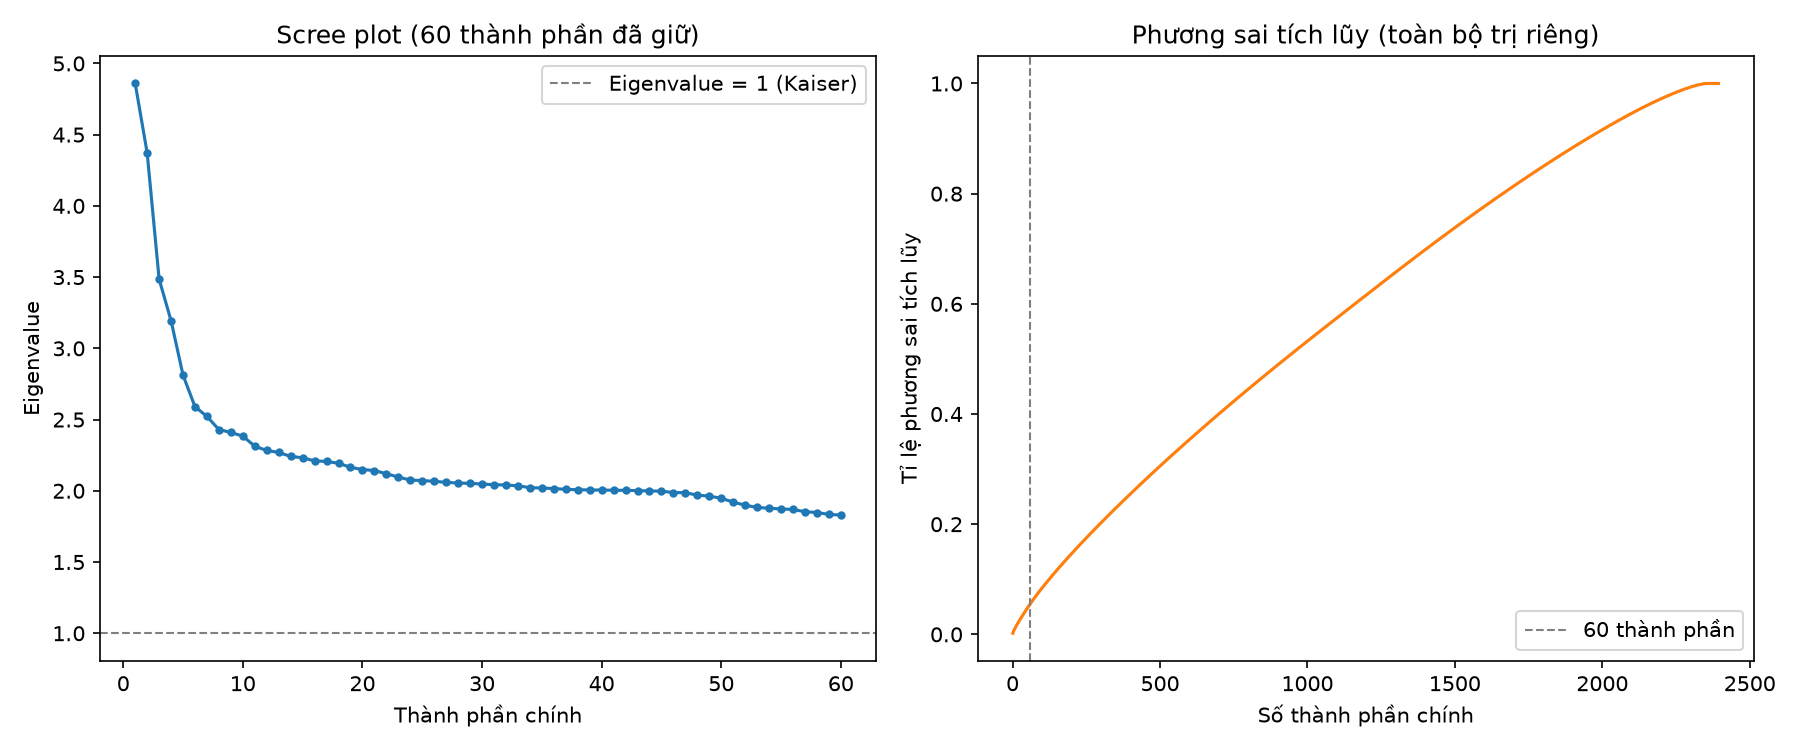
\includegraphics[width=\linewidth,keepaspectratio]{hinh/eigenvalues.png}
  \caption{Scree plot và phương sai tích lũy}
\end{figure}

\begin{itemize}
  \item \textbf{PC1} (eigenvalue 4,8591, giải thích 0,20\% phương sai):

\begin{itemize}
  \item \texttt{change\_\allowbreak{}No}: weight 0,3839
  \item \texttt{change\_\allowbreak{}Ch}: weight -0,3839
  \item \texttt{diabetesMed\_\allowbreak{}No}: weight 0,3618
  \item \texttt{diabetesMed\_\allowbreak{}Yes}: weight -0,3618
  \item \texttt{insulin\_\allowbreak{}No}: weight 0,2756
\end{itemize}

  \item \textbf{PC2} (eigenvalue 4,3718, giải thích 0,18\% phương sai):

\begin{itemize}
  \item \texttt{admission\_\allowbreak{}source\_\allowbreak{}id\_\allowbreak{}7}: weight 0,3591
  \item \texttt{admission\_\allowbreak{}type\_\allowbreak{}id\_\allowbreak{}1}: weight 0,3492
  \item \texttt{admission\_\allowbreak{}source\_\allowbreak{}id\_\allowbreak{}1}: weight -0,3417
  \item \texttt{admission\_\allowbreak{}type\_\allowbreak{}id\_\allowbreak{}3}: weight -0,3065
  \item \texttt{num\_\allowbreak{}lab\_\allowbreak{}procedures}: weight 0,1863
\end{itemize}

  \item \textbf{PC3} (eigenvalue 3,4859, giải thích 0,15\% phương sai):

\begin{itemize}
  \item \texttt{discharge\_\allowbreak{}disposition\_\allowbreak{}id\_\allowbreak{}1}: weight 0,2724
  \item \texttt{num\_\allowbreak{}medications}: weight -0,2306
  \item \texttt{time\_\allowbreak{}in\_\allowbreak{}hospital}: weight -0,2264
  \item \texttt{number\_\allowbreak{}diagnoses}: weight -0,2252
  \item \texttt{num\_\allowbreak{}procedures}: weight -0,1767
\end{itemize}

  \item \textbf{PC4} (eigenvalue 3,1932, giải thích 0,13\% phương sai):

\begin{itemize}
  \item \texttt{diag\_\allowbreak{}2\_\allowbreak{}648}: weight -0,2890
  \item \texttt{medical\_\allowbreak{}specialty\_\allowbreak{}ObstetricsandGynecology}: weight -0,2853
  \item \texttt{diag\_\allowbreak{}1\_\allowbreak{}648}: weight -0,2010
  \item \texttt{age\_\allowbreak{}[20-30)}: weight -0,1788
  \item \texttt{diag\_\allowbreak{}3\_\allowbreak{}648}: weight -0,1676
\end{itemize}

  \item \textbf{PC5} (eigenvalue 2,8114, giải thích 0,12\% phương sai):

\begin{itemize}
  \item \texttt{gender\_\allowbreak{}Male}: weight 0,2328
  \item \texttt{gender\_\allowbreak{}Female}: weight -0,2328
  \item \texttt{num\_\allowbreak{}procedures}: weight 0,2291
  \item \texttt{discharge\_\allowbreak{}disposition\_\allowbreak{}id\_\allowbreak{}1}: weight 0,2178
  \item \texttt{diag\_\allowbreak{}1\_\allowbreak{}414}: weight 0,2100
\end{itemize}
\end{itemize}

\section{CẤU HÌNH THỰC NGHIỆM VÀ HYPERPARAMETER TỐI ƯU}

\subsection{Cấu hình chung}

Quy trình chọn hyperparameter, \texttt{random\_\allowbreak{}state = 42} và phiên bản thư viện: xem 3.1.1 và 3.1.6. Cấu hình chung nêu ở bảng~\ref{tb:chung}.

{\small\setstretch{1.0}\renewcommand\arraystretch{1.1}\setlength\tabcolsep{3pt}
\begin{longtable}{|>{\raggedright\arraybackslash}p{133.52pt}|>{\raggedright\arraybackslash}p{307.52pt}|}
\caption{Cấu hình chung của thực nghiệm}\label{tb:chung}\\
\hline
\textbf{Mục} & \textbf{Giá trị} \\ \hline\endfirsthead
\caption[]{Cấu hình chung của thực nghiệm (tiếp theo)}\\
\hline
\textbf{Mục} & \textbf{Giá trị} \\ \hline\endhead
Dữ liệu vào mô hình & 60 principal component (PCA từ 2.394 cột One-Hot), scale \texttt{StandardScaler} fit trên train (bước 06) cho MLP, Logistic Regression; Decision Tree và Random Forest dùng 60 PC chưa scale (cây không đổi khi co giãn từng cột) \\ \hline
Train / Test & 79.726 / 20.518 lượt nhập viện (chia theo bệnh nhân, bước 03) \\ \hline
Train con / Validation & 63.780 / 15.946 (20\% train, \texttt{random\_\allowbreak{}state = 42}). DT, RF, MLP, LR: stratified theo \texttt{y\_\allowbreak{}bin}, dùng chung một cách chia cho cả hai nhãn để Ensemble dùng được xác suất validation của các mô hình. k-NN và Softmax (3.1.6): stratified theo \texttt{y\_\allowbreak{}multi}, cùng kích thước nhưng khác các dòng được chọn \\ \hline
Nhãn & \texttt{y\_\allowbreak{}multi} $\in$ \{\texttt{<30}, \texttt{>30}, \texttt{NO}\} và \texttt{y\_\allowbreak{}bin} (1 = tái nhập viện) \\ \hline
Độ đo chọn hyperparameter & \texttt{y\_\allowbreak{}multi}: macro-F1; \texttt{y\_\allowbreak{}bin}: AUC-ROC (trên validation) \\ \hline
\end{longtable}
}

Vì vậy điểm validation của k-NN và Softmax không so sánh trực tiếp với DT, RF, MLP; việc so sánh giữa các mô hình dựa vào điểm test (3.3, 3.4).

\subsection{Decision Tree}

Cấu hình quét của Decision Tree nêu ở bảng~\ref{tb:dtcfg}:

{\small\setstretch{1.0}\renewcommand\arraystretch{1.1}\setlength\tabcolsep{3pt}
\begin{longtable}{|>{\raggedright\arraybackslash}p{124.79pt}|>{\raggedright\arraybackslash}p{214.82pt}|}
\caption{Cấu hình quét hyperparameter của Decision Tree}\label{tb:dtcfg}\\
\hline
\textbf{Tham số} & \textbf{Giá trị} \\ \hline\endfirsthead
\caption[]{Cấu hình quét hyperparameter của Decision Tree (tiếp theo)}\\
\hline
\textbf{Tham số} & \textbf{Giá trị} \\ \hline\endhead
Cài đặt & \texttt{sklearn.tree.DecisionTreeClassifier} \\ \hline
Tiêu chí tách & \texttt{gini} (mặc định) \\ \hline
Quét \texttt{max\_\allowbreak{}depth} & 2, 3, ..., 20 và \texttt{None} (20 mức) \\ \hline
Quét \texttt{min\_\allowbreak{}samples\_\allowbreak{}leaf} & 1, 20, 100 \\ \hline
Số cấu hình mỗi nhãn & 60 (20 × 3) \\ \hline
Ngẫu nhiên & \texttt{random\_\allowbreak{}state = 42} \\ \hline
\end{longtable}
}

Hyperparameter tối ưu, trình bày ở bảng~\ref{tb:dtbest}:

{\footnotesize\setstretch{1.0}\renewcommand\arraystretch{1.1}\setlength\tabcolsep{3pt}
\begin{longtable}{|>{\raggedright\arraybackslash}p{40.81pt}|>{\centering\arraybackslash}p{52.19pt}|>{\centering\arraybackslash}p{60.47pt}|>{\raggedright\arraybackslash}p{48.61pt}|>{\centering\arraybackslash}p{30.79pt}|>{\centering\arraybackslash}p{48.84pt}|>{\centering\arraybackslash}p{60.47pt}|>{\centering\arraybackslash}p{60.47pt}|}
\caption{Hyperparameter tối ưu của Decision Tree}\label{tb:dtbest}\\
\hline
\textbf{Nhãn} & \textbf{\texttt{max\_\allowbreak{}depth}} & \textbf{\texttt{min\_\allowbreak{}samples\_\allowbreak{}leaf}} & \textbf{Độ đo} & \textbf{Train} & \textbf{Validation} & \textbf{Test Accuracy} & \textbf{Test (macro-F1 / AUC)} \\ \hline\endfirsthead
\caption[]{Hyperparameter tối ưu của Decision Tree (tiếp theo)}\\
\hline
\textbf{Nhãn} & \textbf{\texttt{max\_\allowbreak{}depth}} & \textbf{\texttt{min\_\allowbreak{}samples\_\allowbreak{}leaf}} & \textbf{Độ đo} & \textbf{Train} & \textbf{Validation} & \textbf{Test Accuracy} & \textbf{Test (macro-F1 / AUC)} \\ \hline\endhead
\texttt{y\_\allowbreak{}multi} & 20 & 1 & macro-F1 & 0,8675 & 0,3717 & 0,4703 & 0,3662 \\ \hline
\texttt{y\_\allowbreak{}bin} & 8 & 100 & AUC-ROC & 0,6580 & 0,6162 & 0,5876 & 0,6140 \\ \hline
\end{longtable}
}

Cột Train và Validation là điểm của mô hình fit trên train con; cột Test là mô hình huấn luyện lại trên toàn bộ train.

Toàn bộ lưới quét cho \texttt{y\_\allowbreak{}multi} (độ đo macro-F1 trên validation; cột là \texttt{min\_\allowbreak{}samples\_\allowbreak{}leaf}), trình bày ở bảng~\ref{tb:dtgridm}:

{\small\setstretch{1.0}\renewcommand\arraystretch{1.1}\setlength\tabcolsep{3pt}
\begin{longtable}{|>{\centering\arraybackslash}p{57.05pt}|>{\centering\arraybackslash}p{68.70pt}|>{\centering\arraybackslash}p{33.62pt}|>{\centering\arraybackslash}p{33.62pt}|}
\caption{Lưới quét của Decision Tree cho bài toán đa lớp (macro-F1 trên validation)}\label{tb:dtgridm}\\
\hline
\textbf{\texttt{max\_\allowbreak{}depth}} & \textbf{1} & \textbf{20} & \textbf{100} \\ \hline\endfirsthead
\caption[]{Lưới quét của Decision Tree cho bài toán đa lớp (macro-F1 trên validation) (tiếp theo)}\\
\hline
\textbf{\texttt{max\_\allowbreak{}depth}} & \textbf{1} & \textbf{20} & \textbf{100} \\ \hline\endhead
2 & 0,3421 & 0,3421 & 0,3421 \\ \hline
3 & 0,3161 & 0,3161 & 0,3161 \\ \hline
4 & 0,3178 & 0,3180 & 0,3162 \\ \hline
5 & 0,3285 & 0,3285 & 0,3269 \\ \hline
6 & 0,3392 & 0,3392 & 0,3375 \\ \hline
7 & 0,3397 & 0,3404 & 0,3367 \\ \hline
8 & 0,3455 & 0,3465 & 0,3435 \\ \hline
9 & 0,3480 & 0,3475 & 0,3395 \\ \hline
10 & 0,3494 & 0,3522 & 0,3420 \\ \hline
11 & 0,3492 & 0,3520 & 0,3425 \\ \hline
12 & 0,3672 & 0,3645 & 0,3495 \\ \hline
13 & 0,3623 & 0,3600 & 0,3443 \\ \hline
14 & 0,3665 & 0,3645 & 0,3491 \\ \hline
15 & 0,3661 & 0,3664 & 0,3494 \\ \hline
16 & 0,3716 & 0,3675 & 0,3485 \\ \hline
17 & 0,3696 & 0,3679 & 0,3494 \\ \hline
18 & 0,3686 & 0,3675 & 0,3491 \\ \hline
19 & 0,3667 & 0,3672 & 0,3491 \\ \hline
20 & 0,3717 \textbf{(chọn)} & 0,3680 & 0,3491 \\ \hline
None & 0,3686 & 0,3697 & 0,3491 \\ \hline
\end{longtable}
}

Toàn bộ lưới quét cho \texttt{y\_\allowbreak{}bin} (độ đo AUC-ROC trên validation; cột là \texttt{min\_\allowbreak{}samples\_\allowbreak{}leaf}), trình bày ở bảng~\ref{tb:dtgridb}:

{\small\setstretch{1.0}\renewcommand\arraystretch{1.1}\setlength\tabcolsep{3pt}
\begin{longtable}{|>{\centering\arraybackslash}p{57.05pt}|>{\centering\arraybackslash}p{33.62pt}|>{\centering\arraybackslash}p{33.62pt}|>{\centering\arraybackslash}p{68.70pt}|}
\caption{Lưới quét của Decision Tree cho bài toán nhị phân (AUC-ROC trên validation)}\label{tb:dtgridb}\\
\hline
\textbf{\texttt{max\_\allowbreak{}depth}} & \textbf{1} & \textbf{20} & \textbf{100} \\ \hline\endfirsthead
\caption[]{Lưới quét của Decision Tree cho bài toán nhị phân (AUC-ROC trên validation) (tiếp theo)}\\
\hline
\textbf{\texttt{max\_\allowbreak{}depth}} & \textbf{1} & \textbf{20} & \textbf{100} \\ \hline\endhead
2 & 0,5642 & 0,5642 & 0,5642 \\ \hline
3 & 0,5821 & 0,5821 & 0,5821 \\ \hline
4 & 0,5959 & 0,5960 & 0,5958 \\ \hline
5 & 0,6049 & 0,6057 & 0,6058 \\ \hline
6 & 0,6088 & 0,6096 & 0,6111 \\ \hline
7 & 0,6079 & 0,6093 & 0,6111 \\ \hline
8 & 0,6097 & 0,6098 & 0,6162 \textbf{(chọn)} \\ \hline
9 & 0,6018 & 0,6042 & 0,6133 \\ \hline
10 & 0,5984 & 0,5994 & 0,6108 \\ \hline
11 & 0,5965 & 0,6002 & 0,6089 \\ \hline
12 & 0,5885 & 0,5965 & 0,6070 \\ \hline
13 & 0,5790 & 0,5926 & 0,6066 \\ \hline
14 & 0,5746 & 0,5895 & 0,6046 \\ \hline
15 & 0,5645 & 0,5848 & 0,6045 \\ \hline
16 & 0,5567 & 0,5839 & 0,6047 \\ \hline
17 & 0,5513 & 0,5823 & 0,6047 \\ \hline
18 & 0,5449 & 0,5798 & 0,6047 \\ \hline
19 & 0,5473 & 0,5772 & 0,6047 \\ \hline
20 & 0,5444 & 0,5776 & 0,6047 \\ \hline
None & 0,5430 & 0,5755 & 0,6047 \\ \hline
\end{longtable}
}

\subsection{Random Forest}

Cấu hình quét của Random Forest nêu ở bảng~\ref{tb:rfcfg}:

{\small\setstretch{1.0}\renewcommand\arraystretch{1.1}\setlength\tabcolsep{3pt}
\begin{longtable}{|>{\raggedright\arraybackslash}p{104.47pt}|>{\raggedright\arraybackslash}p{336.57pt}|}
\caption{Cấu hình quét hyperparameter của Random Forest}\label{tb:rfcfg}\\
\hline
\textbf{Tham số} & \textbf{Giá trị} \\ \hline\endfirsthead
\caption[]{Cấu hình quét hyperparameter của Random Forest (tiếp theo)}\\
\hline
\textbf{Tham số} & \textbf{Giá trị} \\ \hline\endhead
Cài đặt & \texttt{sklearn.ensemble.RandomForestClassifier} \\ \hline
\texttt{max\_\allowbreak{}features} & \texttt{sqrt} (mặc định) \\ \hline
\texttt{min\_\allowbreak{}samples\_\allowbreak{}leaf} & 1 (mặc định) \\ \hline
Quét \texttt{n\_\allowbreak{}estimators} & 50, 100, 200, 400 \\ \hline
Quét \texttt{max\_\allowbreak{}depth} & 4, 6, 8, 10, 12, 16, 20, \texttt{None} \\ \hline
Số cấu hình mỗi nhãn & 32 (4 × 8) \\ \hline
Cách quét & Với mỗi \texttt{max\_\allowbreak{}depth} huấn luyện một rừng 400 cây rồi đánh giá trên 50, 100, 200 cây đầu (đã kiểm tra tương đương huấn luyện riêng bằng \texttt{assert}) \\ \hline
Ngẫu nhiên & \texttt{random\_\allowbreak{}state = 42} \\ \hline
\end{longtable}
}

Hyperparameter tối ưu, trình bày ở bảng~\ref{tb:rfbest}:

{\footnotesize\setstretch{1.0}\renewcommand\arraystretch{1.1}\setlength\tabcolsep{3pt}
\begin{longtable}{|>{\raggedright\arraybackslash}p{40.81pt}|>{\centering\arraybackslash}p{60.47pt}|>{\raggedright\arraybackslash}p{52.19pt}|>{\raggedright\arraybackslash}p{48.61pt}|>{\centering\arraybackslash}p{30.79pt}|>{\centering\arraybackslash}p{48.84pt}|>{\centering\arraybackslash}p{60.47pt}|>{\centering\arraybackslash}p{60.47pt}|}
\caption{Hyperparameter tối ưu của Random Forest}\label{tb:rfbest}\\
\hline
\textbf{Nhãn} & \textbf{\texttt{n\_\allowbreak{}estimators}} & \textbf{\texttt{max\_\allowbreak{}depth}} & \textbf{Độ đo} & \textbf{Train} & \textbf{Validation} & \textbf{Test Accuracy} & \textbf{Test (macro-F1 / AUC)} \\ \hline\endfirsthead
\caption[]{Hyperparameter tối ưu của Random Forest (tiếp theo)}\\
\hline
\textbf{Nhãn} & \textbf{\texttt{n\_\allowbreak{}estimators}} & \textbf{\texttt{max\_\allowbreak{}depth}} & \textbf{Độ đo} & \textbf{Train} & \textbf{Validation} & \textbf{Test Accuracy} & \textbf{Test (macro-F1 / AUC)} \\ \hline\endhead
\texttt{y\_\allowbreak{}multi} & 50 & None & macro-F1 & 1,0000 & 0,3653 & 0,5492 & 0,3587 \\ \hline
\texttt{y\_\allowbreak{}bin} & 400 & 20 & AUC-ROC & 1,0000 & 0,6542 & 0,6085 & 0,6537 \\ \hline
\end{longtable}
}

Cột Train và Validation là điểm của mô hình fit trên train con; cột Test là mô hình huấn luyện lại trên toàn bộ train.

Toàn bộ lưới quét cho \texttt{y\_\allowbreak{}multi} (độ đo macro-F1 trên validation; cột là \texttt{n\_\allowbreak{}estimators}), trình bày ở bảng~\ref{tb:rfgridm}:

{\small\setstretch{1.0}\renewcommand\arraystretch{1.1}\setlength\tabcolsep{3pt}
\begin{longtable}{|>{\centering\arraybackslash}p{57.05pt}|>{\centering\arraybackslash}p{68.70pt}|>{\centering\arraybackslash}p{33.62pt}|>{\centering\arraybackslash}p{33.62pt}|>{\centering\arraybackslash}p{33.62pt}|}
\caption{Lưới quét của Random Forest cho bài toán đa lớp (macro-F1 trên validation)}\label{tb:rfgridm}\\
\hline
\textbf{\texttt{max\_\allowbreak{}depth}} & \textbf{50} & \textbf{100} & \textbf{200} & \textbf{400} \\ \hline\endfirsthead
\caption[]{Lưới quét của Random Forest cho bài toán đa lớp (macro-F1 trên validation) (tiếp theo)}\\
\hline
\textbf{\texttt{max\_\allowbreak{}depth}} & \textbf{50} & \textbf{100} & \textbf{200} & \textbf{400} \\ \hline\endhead
4 & 0,2500 & 0,2499 & 0,2516 & 0,2498 \\ \hline
6 & 0,2894 & 0,2916 & 0,2891 & 0,2894 \\ \hline
8 & 0,3201 & 0,3169 & 0,3166 & 0,3163 \\ \hline
10 & 0,3361 & 0,3327 & 0,3326 & 0,3322 \\ \hline
12 & 0,3456 & 0,3430 & 0,3439 & 0,3430 \\ \hline
16 & 0,3541 & 0,3516 & 0,3515 & 0,3519 \\ \hline
20 & 0,3639 & 0,3606 & 0,3590 & 0,3565 \\ \hline
None & 0,3653 \textbf{(chọn)} & 0,3646 & 0,3634 & 0,3581 \\ \hline
\end{longtable}
}

Toàn bộ lưới quét cho \texttt{y\_\allowbreak{}bin} (độ đo AUC-ROC trên validation; cột là \texttt{n\_\allowbreak{}estimators}), trình bày ở bảng~\ref{tb:rfgridb}:

{\small\setstretch{1.0}\renewcommand\arraystretch{1.1}\setlength\tabcolsep{3pt}
\begin{longtable}{|>{\centering\arraybackslash}p{57.05pt}|>{\centering\arraybackslash}p{33.62pt}|>{\centering\arraybackslash}p{33.62pt}|>{\centering\arraybackslash}p{33.62pt}|>{\centering\arraybackslash}p{68.70pt}|}
\caption{Lưới quét của Random Forest cho bài toán nhị phân (AUC-ROC trên validation)}\label{tb:rfgridb}\\
\hline
\textbf{\texttt{max\_\allowbreak{}depth}} & \textbf{50} & \textbf{100} & \textbf{200} & \textbf{400} \\ \hline\endfirsthead
\caption[]{Lưới quét của Random Forest cho bài toán nhị phân (AUC-ROC trên validation) (tiếp theo)}\\
\hline
\textbf{\texttt{max\_\allowbreak{}depth}} & \textbf{50} & \textbf{100} & \textbf{200} & \textbf{400} \\ \hline\endhead
4 & 0,6301 & 0,6310 & 0,6303 & 0,6308 \\ \hline
6 & 0,6381 & 0,6394 & 0,6394 & 0,6396 \\ \hline
8 & 0,6438 & 0,6449 & 0,6456 & 0,6457 \\ \hline
10 & 0,6466 & 0,6481 & 0,6501 & 0,6503 \\ \hline
12 & 0,6465 & 0,6483 & 0,6517 & 0,6527 \\ \hline
16 & 0,6419 & 0,6483 & 0,6514 & 0,6533 \\ \hline
20 & 0,6380 & 0,6474 & 0,6517 & 0,6542 \textbf{(chọn)} \\ \hline
None & 0,6301 & 0,6412 & 0,6493 & 0,6530 \\ \hline
\end{longtable}
}

\textbf{Nhận xét.} Với Decision Tree \texttt{y\_\allowbreak{}bin}, điểm validation tăng đến \texttt{max\_\allowbreak{}depth} 6–8 rồi giảm: cấu hình tốt nhất (\texttt{max\_\allowbreak{}depth = 8}, \texttt{min\_\allowbreak{}samples\_\allowbreak{}leaf = 100}) đạt 0,6162, còn cây không giới hạn độ sâu với \texttt{min\_\allowbreak{}samples\_\allowbreak{}leaf = 1} chỉ đạt 0,5430 trong khi điểm train gần 1, tức là overfit rõ; \texttt{min\_\allowbreak{}samples\_\allowbreak{}leaf} lớn giúp cây sâu giảm overfit (0,5430 lên 0,6047 ở \texttt{max\_\allowbreak{}depth = None}). Với \texttt{y\_\allowbreak{}multi}, từ \texttt{max\_\allowbreak{}depth} 12 trở đi điểm validation dao động trong khoảng hẹp 0,360–0,372 (với \texttt{min\_\allowbreak{}samples\_\allowbreak{}leaf} bằng 1 hoặc 20) nên lựa chọn ít quan trọng. Với Random Forest \texttt{y\_\allowbreak{}bin}, độ sâu tối ưu phụ thuộc số cây: với 50 cây điểm cao nhất ở \texttt{max\_\allowbreak{}depth} 10–12 (0,6466) rồi giảm dần khi cây sâu hơn, còn với 400 cây đỉnh dịch sang \texttt{max\_\allowbreak{}depth = 20} (0,6542) và chỉ giảm nhẹ ở \texttt{None} (0,6530); thêm cây cho phép rừng sâu hơn mà không overfit (ở \texttt{max\_\allowbreak{}depth = 20}, AUC tăng từ 0,6380 lên 0,6542 khi \texttt{n\_\allowbreak{}estimators} từ 50 lên 400). Với \texttt{y\_\allowbreak{}multi} thêm cây không cải thiện mà còn làm macro-F1 validation giảm nhẹ (khoảng 0,007 ở \texttt{max\_\allowbreak{}depth = 20} và \texttt{None}), nên cấu hình tốt nhất dùng 50 cây. Cả hai mô hình đều khó nhận ra lớp \texttt{<30}, nên macro-F1 của \texttt{y\_\allowbreak{}multi} chỉ khoảng 0,36.

\subsection{MLP 120-60-20}

Tham số cố định và lưới quét, trình bày ở bảng~\ref{tb:mlpcfg}:

{\small\setstretch{1.0}\renewcommand\arraystretch{1.1}\setlength\tabcolsep{3pt}
\begin{longtable}{|>{\raggedright\arraybackslash}p{137.00pt}|>{\raggedright\arraybackslash}p{304.04pt}|}
\caption{Tham số cố định và lưới quét của MLP}\label{tb:mlpcfg}\\
\hline
\textbf{Tham số} & \textbf{Giá trị} \\ \hline\endfirsthead
\caption[]{Tham số cố định và lưới quét của MLP (tiếp theo)}\\
\hline
\textbf{Tham số} & \textbf{Giá trị} \\ \hline\endhead
Cài đặt & \texttt{sklearn.neural\_\allowbreak{}network.MLPClassifier} \\ \hline
Lớp ẩn & (120, 60, 20), kích hoạt ReLU \\ \hline
Bộ tối ưu & Adam, \texttt{max\_\allowbreak{}iter = 300} \\ \hline
Early stopping & \texttt{early\_\allowbreak{}stopping=True}, \texttt{validation\_\allowbreak{}fraction=0.1}, \texttt{n\_\allowbreak{}iter\_\allowbreak{}no\_\allowbreak{}change=10} \\ \hline
Quét \texttt{alpha} (L2) & 1e-5, 1e-4, 1e-3, 1e-2, 1e-1, 1 \\ \hline
Quét \texttt{learning\_\allowbreak{}rate\_\allowbreak{}init} & 1e-3, 1e-2 \\ \hline
Số cấu hình mỗi nhãn & 12 (6 × 2) \\ \hline
\end{longtable}
}

Hyperparameter tối ưu, trình bày ở bảng~\ref{tb:mlpbest}:

{\footnotesize\setstretch{1.0}\renewcommand\arraystretch{1.1}\setlength\tabcolsep{3pt}
\begin{longtable}{|>{\raggedright\arraybackslash}p{40.81pt}|>{\centering\arraybackslash}p{30.79pt}|>{\centering\arraybackslash}p{68.31pt}|>{\raggedright\arraybackslash}p{48.61pt}|>{\centering\arraybackslash}p{30.79pt}|>{\centering\arraybackslash}p{48.84pt}|>{\centering\arraybackslash}p{66.18pt}|>{\centering\arraybackslash}p{68.31pt}|}
\caption{Hyperparameter tối ưu của MLP}\label{tb:mlpbest}\\
\hline
\textbf{Nhãn} & \textbf{\texttt{alpha}} & \textbf{\texttt{learning\_\allowbreak{}rate\_\allowbreak{}init}} & \textbf{Độ đo} & \textbf{Train} & \textbf{Validation} & \textbf{Test Accuracy} & \textbf{Test (macro-F1 / AUC)} \\ \hline\endfirsthead
\caption[]{Hyperparameter tối ưu của MLP (tiếp theo)}\\
\hline
\textbf{Nhãn} & \textbf{\texttt{alpha}} & \textbf{\texttt{learning\_\allowbreak{}rate\_\allowbreak{}init}} & \textbf{Độ đo} & \textbf{Train} & \textbf{Validation} & \textbf{Test Accuracy} & \textbf{Test (macro-F1 / AUC)} \\ \hline\endhead
\texttt{y\_\allowbreak{}multi} & 0,0001 & 0,01 & macro-F1 & 0,3892 & 0,3753 & 0,5647 & 0,3591 \\ \hline
\texttt{y\_\allowbreak{}bin} & 0,1 & 0,001 & AUC-ROC & 0,6989 & 0,6706 & 0,6212 & 0,6683 \\ \hline
\end{longtable}
}

Cột Train và Validation là điểm của mô hình fit trên train con; cột Test là mô hình huấn luyện lại trên toàn bộ train.

Toàn bộ lưới quét cho \texttt{y\_\allowbreak{}multi} (độ đo macro-F1; số epoch là số lần lặp thực tế trước khi early stopping dừng), trình bày ở bảng~\ref{tb:mlpgridm}:

{\small\setstretch{1.0}\renewcommand\arraystretch{1.1}\setlength\tabcolsep{3pt}
\begin{longtable}{|>{\centering\arraybackslash}p{33.62pt}|>{\centering\arraybackslash}p{113.10pt}|>{\centering\arraybackslash}p{33.62pt}|>{\centering\arraybackslash}p{68.70pt}|>{\centering\arraybackslash}p{45.97pt}|}
\caption{Lưới quét của MLP cho bài toán đa lớp (macro-F1 trên validation)}\label{tb:mlpgridm}\\
\hline
\textbf{\texttt{alpha}} & \textbf{\texttt{learning\_\allowbreak{}rate\_\allowbreak{}init}} & \textbf{Train} & \textbf{Validation} & \textbf{Số epoch} \\ \hline\endfirsthead
\caption[]{Lưới quét của MLP cho bài toán đa lớp (macro-F1 trên validation) (tiếp theo)}\\
\hline
\textbf{\texttt{alpha}} & \textbf{\texttt{learning\_\allowbreak{}rate\_\allowbreak{}init}} & \textbf{Train} & \textbf{Validation} & \textbf{Số epoch} \\ \hline\endhead
1e-05 & 0,001 & 0,3720 & 0,3606 & 16 \\ \hline
0,0001 & 0,001 & 0,3737 & 0,3616 & 16 \\ \hline
0,001 & 0,001 & 0,3865 & 0,3708 & 17 \\ \hline
0,01 & 0,001 & 0,3759 & 0,3644 & 16 \\ \hline
0,1 & 0,001 & 0,3881 & 0,3673 & 35 \\ \hline
1 & 0,001 & 0,3655 & 0,3582 & 32 \\ \hline
1e-05 & 0,01 & 0,3797 & 0,3683 & 28 \\ \hline
0,0001 & 0,01 & 0,3892 & 0,3753 \textbf{(chọn)} & 25 \\ \hline
0,001 & 0,01 & 0,3910 & 0,3724 & 22 \\ \hline
0,01 & 0,01 & 0,3868 & 0,3750 & 32 \\ \hline
0,1 & 0,01 & 0,3753 & 0,3698 & 18 \\ \hline
1 & 0,01 & 0,3493 & 0,3481 & 20 \\ \hline
\end{longtable}
}

Toàn bộ lưới quét cho \texttt{y\_\allowbreak{}bin} (độ đo AUC-ROC; số epoch là số lần lặp thực tế trước khi early stopping dừng), trình bày ở bảng~\ref{tb:mlpgridb}:

{\small\setstretch{1.0}\renewcommand\arraystretch{1.1}\setlength\tabcolsep{3pt}
\begin{longtable}{|>{\centering\arraybackslash}p{33.62pt}|>{\centering\arraybackslash}p{113.10pt}|>{\centering\arraybackslash}p{33.62pt}|>{\centering\arraybackslash}p{68.70pt}|>{\centering\arraybackslash}p{45.97pt}|}
\caption{Lưới quét của MLP cho bài toán nhị phân (AUC-ROC trên validation)}\label{tb:mlpgridb}\\
\hline
\textbf{\texttt{alpha}} & \textbf{\texttt{learning\_\allowbreak{}rate\_\allowbreak{}init}} & \textbf{Train} & \textbf{Validation} & \textbf{Số epoch} \\ \hline\endfirsthead
\caption[]{Lưới quét của MLP cho bài toán nhị phân (AUC-ROC trên validation) (tiếp theo)}\\
\hline
\textbf{\texttt{alpha}} & \textbf{\texttt{learning\_\allowbreak{}rate\_\allowbreak{}init}} & \textbf{Train} & \textbf{Validation} & \textbf{Số epoch} \\ \hline\endhead
1e-05 & 0,001 & 0,6989 & 0,6650 & 19 \\ \hline
0,0001 & 0,001 & 0,6996 & 0,6635 & 19 \\ \hline
0,001 & 0,001 & 0,7272 & 0,6624 & 28 \\ \hline
0,01 & 0,001 & 0,7240 & 0,6632 & 28 \\ \hline
0,1 & 0,001 & 0,6989 & 0,6706 \textbf{(chọn)} & 28 \\ \hline
1 & 0,001 & 0,6575 & 0,6515 & 28 \\ \hline
1e-05 & 0,01 & 0,6834 & 0,6619 & 18 \\ \hline
0,0001 & 0,01 & 0,6885 & 0,6659 & 19 \\ \hline
0,001 & 0,01 & 0,6825 & 0,6623 & 19 \\ \hline
0,01 & 0,01 & 0,6772 & 0,6622 & 19 \\ \hline
0,1 & 0,01 & 0,6641 & 0,6522 & 22 \\ \hline
1 & 0,01 & 0,6351 & 0,6333 & 12 \\ \hline
\end{longtable}
}

\textbf{Nhận xét.} Với \texttt{y\_\allowbreak{}bin}, điểm validation của 12 cấu hình chỉ dao động từ 0,6333 đến 0,6706 (khoảng 0,0373), nên việc chọn hyperparameter có ảnh hưởng nhỏ. \texttt{alpha = 1} (phạt L2 mạnh nhất) cho điểm thấp nhất ở cả hai learning rate, vì mô hình bị ép về hàm quá đơn giản (underfit). Bài báo tham khảo tìm được alpha tốt nhất là 1e-4; ở đây \texttt{y\_\allowbreak{}multi} chọn đúng 1e-4 còn \texttt{y\_\allowbreak{}bin} chọn 1e-1.

Trên \texttt{y\_\allowbreak{}multi}, MLP đạt Test Accuracy 0,5647 và macro-F1 0,3591. Mốc “luôn đoán \texttt{NO}” có accuracy 0,5323, nên MLP chỉ hơn mốc 3,2 điểm phần trăm; macro-F1 xấp xỉ Random Forest (0,3587) và Softmax chưa scale (0,3595), thấp hơn k-NN chưa scale (0,3807) và Decision Tree (0,3662). Kết quả nhị phân của MLP là tốt nhất trong các mô hình đơn (3.4).

\subsection{Aggregate Ensemble theo weight AUC-ROC}

Cấu hình của Ensemble nêu ở bảng~\ref{tb:enscfg}:

{\small\setstretch{1.0}\renewcommand\arraystretch{1.1}\setlength\tabcolsep{3pt}
\begin{longtable}{|>{\raggedright\arraybackslash}p{151.88pt}|>{\raggedright\arraybackslash}p{289.16pt}|}
\caption{Cấu hình của Aggregate Ensemble theo weight AUC-ROC}\label{tb:enscfg}\\
\hline
\textbf{Tham số} & \textbf{Giá trị} \\ \hline\endfirsthead
\caption[]{Cấu hình của Aggregate Ensemble theo weight AUC-ROC (tiếp theo)}\\
\hline
\textbf{Tham số} & \textbf{Giá trị} \\ \hline\endhead
Bài toán & Nhị phân (\texttt{y\_\allowbreak{}bin}) \\ \hline
Công thức weight & $w_i = \mathrm{AUC}_i / \sum_j \mathrm{AUC}_j$, AUC tính trên \textbf{validation} \\ \hline
Xác suất ensemble & $p_{\text{ens}} = \sum_i w_i\,p_i$; dự đoán lớp 1 khi $p_{\text{ens}} \ge 0{,}5$ \\ \hline
Thành viên Logistic Regression & \texttt{LogisticRegression(max\_\allowbreak{}iter=1000)}, tham số mặc định khác (\texttt{C = 1}, L2, \texttt{lbfgs}) \\ \hline
Thành viên MLP & Cấu hình tối ưu của \texttt{y\_\allowbreak{}bin} ở trên \\ \hline
Thành viên DT, RF & Cấu hình tối ưu của \texttt{y\_\allowbreak{}bin} ở mục 3.2.2 và 3.2.3, xác suất validation từ mô hình fit trên train con, xác suất test từ mô hình huấn luyện lại trên toàn bộ train \\ \hline
Biến thể so sánh & Trung bình không weight; $w_i \propto \mathrm{AUC}_i - 0{,}5$ \\ \hline
\end{longtable}
}

Weight tính được cho 4 thành viên nêu ở bảng~\ref{tb:wensemble}:

{\small\setstretch{1.0}\renewcommand\arraystretch{1.1}\setlength\tabcolsep{3pt}
\begin{longtable}{|>{\raggedright\arraybackslash}p{44.18pt}|>{\centering\arraybackslash}p{79.35pt}|>{\centering\arraybackslash}p{62.32pt}|>{\centering\arraybackslash}p{33.62pt}|>{\centering\arraybackslash}p{92.41pt}|}
\caption{Weight của bốn thành viên Ensemble}\label{tb:wensemble}\\
\hline
\textbf{Mô hình} & \textbf{AUC validation} & \textbf{$w$ theo AUC} & \textbf{$w$ đều} & \textbf{$w$ theo AUC $-$ 0,5} \\ \hline\endfirsthead
\caption[]{Weight của bốn thành viên Ensemble (tiếp theo)}\\
\hline
\textbf{Mô hình} & \textbf{AUC validation} & \textbf{$w$ theo AUC} & \textbf{$w$ đều} & \textbf{$w$ theo AUC $-$ 0,5} \\ \hline\endhead
DT & 0,6162 & 0,2395 & 0,2500 & 0,2028 \\ \hline
RF & 0,6542 & 0,2543 & 0,2500 & 0,2693 \\ \hline
MLP & 0,6706 & 0,2607 & 0,2500 & 0,2979 \\ \hline
LR & 0,6317 & 0,2456 & 0,2500 & 0,2300 \\ \hline
\end{longtable}
}

Kết quả test của ensemble và từng mô hình đơn: xem 3.4.

\section{BẢNG SO SÁNH KẾT QUẢ THỰC NGHIỆM VÀ CONFUSION MATRIX}

Mục này trình bày kết quả trên \textbf{tập test} (20.518 lượt nhập viện) của bài toán đa lớp \texttt{y\_\allowbreak{}multi} $\in$ \{\texttt{<30}, \texttt{>30}, \texttt{NO}\}, cho hai mô hình k-NN (bước 07a) và Softmax Regression (bước 07b), mỗi mô hình chạy trên hai phiên bản dữ liệu PCA: chưa scale và đã scale (xem 3.1.6). Số liệu được tính từ nhãn dự đoán của bước 07a, 07b, trong lần chạy notebook tổng hợp trên Colab.

\subsection{Bảng so sánh kết quả}

Kết quả so sánh nêu ở bảng~\ref{tb:sosanh}:

{\footnotesize\setstretch{1.0}\renewcommand\arraystretch{1.1}\setlength\tabcolsep{3pt}
\begin{longtable}{|>{\raggedright\arraybackslash}p{72.26pt}|>{\raggedright\arraybackslash}p{48.37pt}|>{\raggedright\arraybackslash}p{79.26pt}|>{\centering\arraybackslash}p{59.18pt}|>{\centering\arraybackslash}p{47.16pt}|>{\centering\arraybackslash}p{32.81pt}|>{\centering\arraybackslash}p{32.81pt}|>{\centering\arraybackslash}p{30.79pt}|}
\caption{So sánh k-NN và Softmax Regression trên tập test (bài toán đa lớp)}\label{tb:sosanh}\\
\hline
\textbf{Mô hình} & \textbf{Dữ liệu} & \textbf{Hyperparameter chọn trên validation} & \textbf{Test Accuracy} & \textbf{Macro-F1} & \textbf{F1 \texttt{<30}} & \textbf{F1 \texttt{>30}} & \textbf{F1 \texttt{NO}} \\ \hline\endfirsthead
\caption[]{So sánh k-NN và Softmax Regression trên tập test (bài toán đa lớp) (tiếp theo)}\\
\hline
\textbf{Mô hình} & \textbf{Dữ liệu} & \textbf{Hyperparameter chọn trên validation} & \textbf{Test Accuracy} & \textbf{Macro-F1} & \textbf{F1 \texttt{<30}} & \textbf{F1 \texttt{>30}} & \textbf{F1 \texttt{NO}} \\ \hline\endhead
k-NN & Chưa scale & $k = 5$ & 0,4860 & \textbf{0,3807} & \textbf{0,1327} & 0,4137 & 0,5956 \\ \hline
k-NN & Đã scale & $k = 9$ & 0,5105 & 0,3718 & 0,0768 & 0,4130 & 0,6256 \\ \hline
Softmax Regression & Chưa scale & lr = 0,001; $\lambda = 0{,}001$ & 0,5337 & 0,3595 & 0,0017 & \textbf{0,4268} & 0,6499 \\ \hline
Softmax Regression & Đã scale & lr = 0,5; $\lambda = 0$ & \textbf{0,5505} & 0,3323 & 0,0008 & 0,3056 & \textbf{0,6906} \\ \hline
\textit{Mốc: luôn đoán \texttt{NO}} & – & – & \textit{0,5323} & \textit{0,2316} & \textit{0} & \textit{0} & \textit{0,6948} \\ \hline
\end{longtable}
}

\textit{Ghi chú:} macro-F1 là trung bình F1 của ba lớp, không weight; đây là độ đo chính để chọn hyperparameter (3.1.6). Dòng mốc được tính từ phân bố nhãn của tập test (10.922 / 20.518 mẫu là \texttt{NO}).

\subsection{Confusion matrix}

\begin{figure}[H]
  \centering
  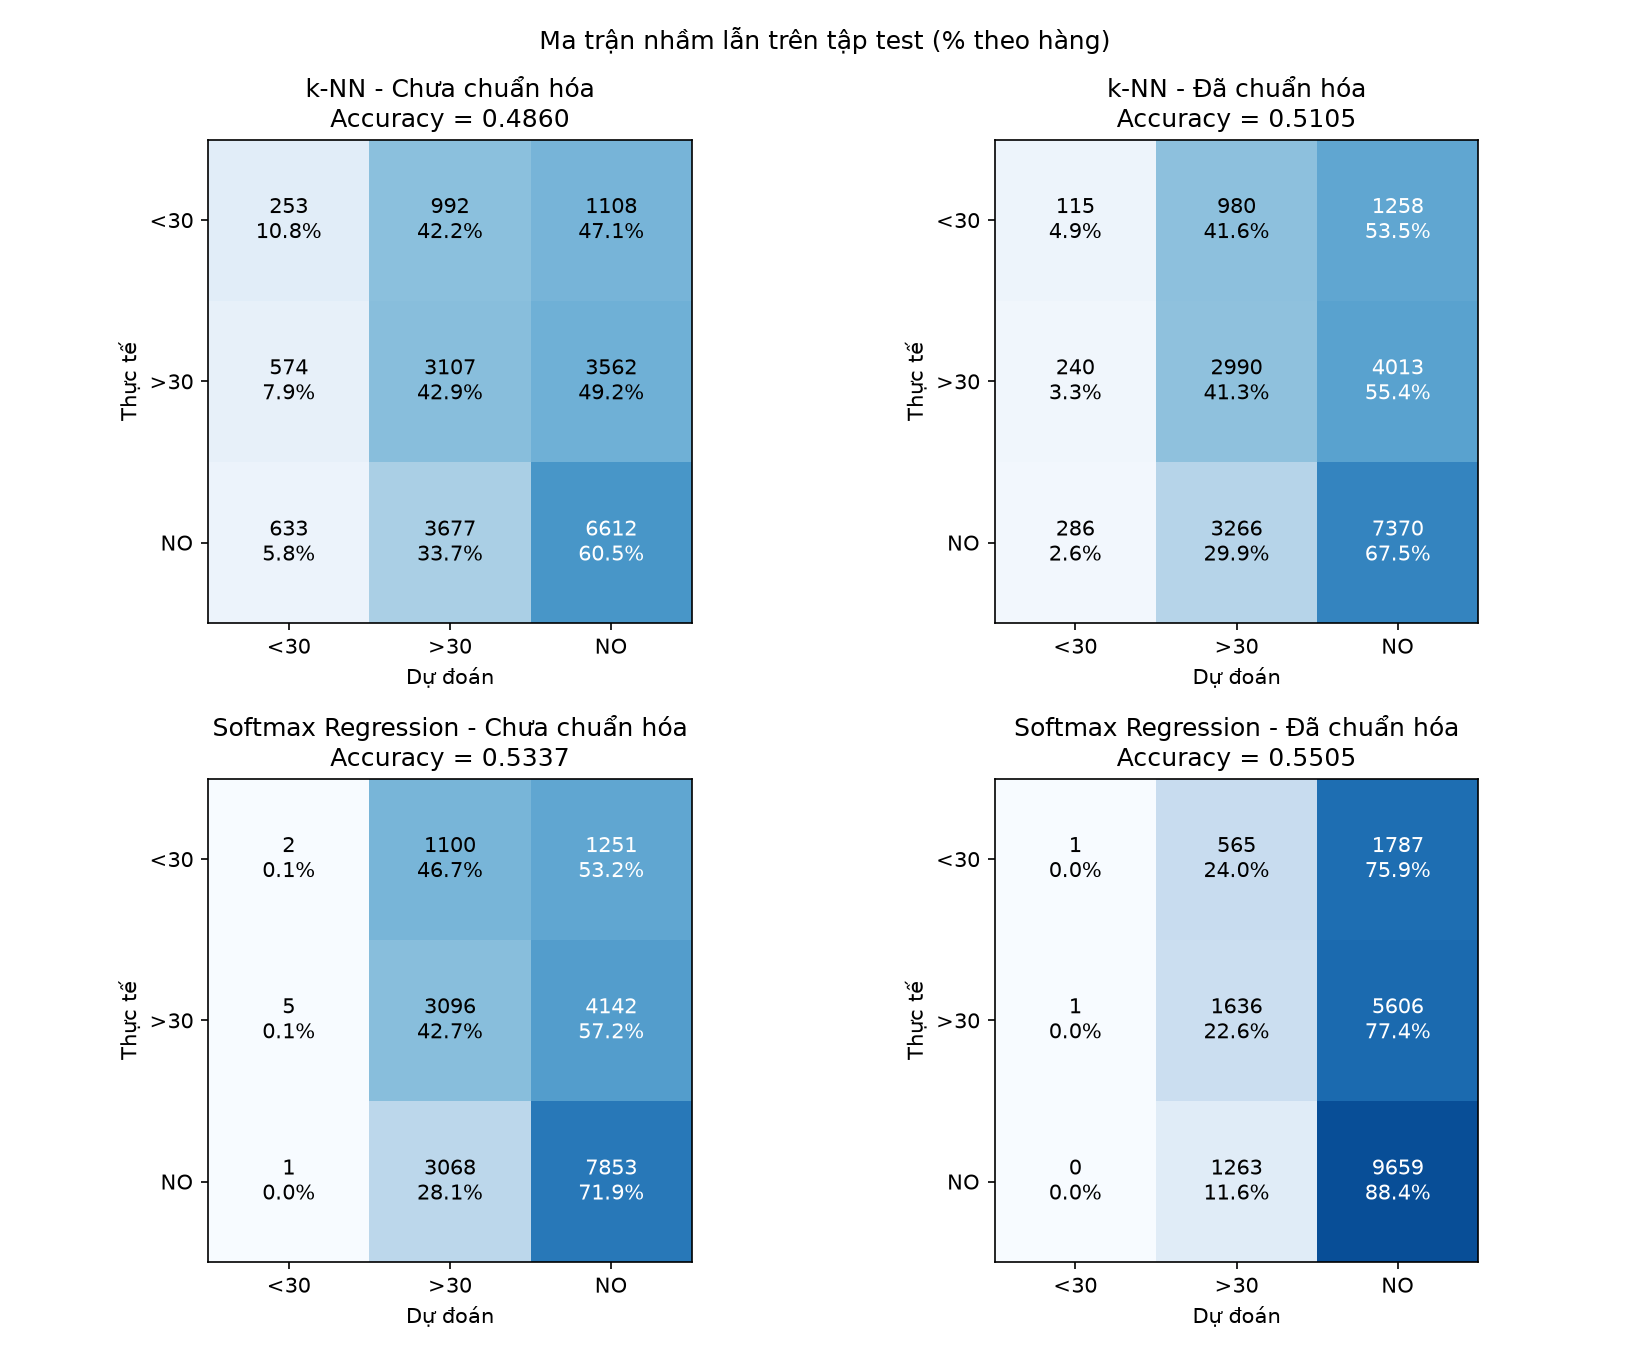
\includegraphics[width=\linewidth,keepaspectratio]{hinh/confusion_matrices.png}
  \caption{Confusion matrix trên tập test}
\end{figure}

\textit{Hình: confusion matrix trên tập test. Hàng là nhãn thực tế, cột là nhãn dự đoán; mỗi ô ghi số mẫu và tỉ lệ phần trăm theo hàng (tức recall của lớp đó ở đường chéo).}

Recall từng lớp (đường chéo ma trận, chia cho tổng hàng) nêu ở bảng~\ref{tb:recall}:

{\footnotesize\setstretch{1.0}\renewcommand\arraystretch{1.1}\setlength\tabcolsep{3pt}
\begin{longtable}{|>{\raggedright\arraybackslash}p{40.43pt}|>{\raggedright\arraybackslash}p{48.37pt}|>{\centering\arraybackslash}p{83.89pt}|>{\centering\arraybackslash}p{83.89pt}|>{\centering\arraybackslash}p{83.89pt}|>{\centering\arraybackslash}p{74.96pt}|}
\caption{Recall từng lớp của k-NN và Softmax Regression trên tập test}\label{tb:recall}\\
\hline
\textbf{Mô hình} & \textbf{Dữ liệu} & \textbf{Recall \texttt{<30} (2.353 mẫu)} & \textbf{Recall \texttt{>30} (7.243 mẫu)} & \textbf{Recall \texttt{NO} (10.922 mẫu)} & \textbf{Số lần đoán \texttt{<30}} \\ \hline\endfirsthead
\caption[]{Recall từng lớp của k-NN và Softmax Regression trên tập test (tiếp theo)}\\
\hline
\textbf{Mô hình} & \textbf{Dữ liệu} & \textbf{Recall \texttt{<30} (2.353 mẫu)} & \textbf{Recall \texttt{>30} (7.243 mẫu)} & \textbf{Recall \texttt{NO} (10.922 mẫu)} & \textbf{Số lần đoán \texttt{<30}} \\ \hline\endhead
k-NN & Chưa scale & 253 (10,8\%) & 3.107 (42,9\%) & 6.612 (60,5\%) & 1.460 \\ \hline
k-NN & Đã scale & 115 (4,9\%) & 2.990 (41,3\%) & 7.370 (67,5\%) & 641 \\ \hline
Softmax & Chưa scale & 2 (0,1\%) & 3.096 (42,7\%) & 7.853 (71,9\%) & 8 \\ \hline
Softmax & Đã scale & 1 (0,0\%) & 1.636 (22,6\%) & 9.659 (88,4\%) & 2 \\ \hline
\end{longtable}
}

\subsection{Nhận xét}

\begin{itemize}
  \item \textbf{Accuracy cao hơn không có nghĩa là mô hình tốt hơn.} Softmax đã scale có accuracy cao nhất (0,5505) nhưng chỉ hơn mốc “luôn đoán \texttt{NO}” (0,5323) khoảng 1,8 điểm phần trăm. Confusion matrix cho thấy lý do: mô hình đoán \texttt{NO} cho 17.052 / 20.518 mẫu (83,1\%), recall lớp \texttt{NO} đạt 88,4\%, còn lớp \texttt{<30} chỉ được đoán 2 lần trên toàn tập test. Ngược lại, k-NN chưa scale có accuracy thấp hơn mốc nhưng macro-F1 cao nhất (0,3807), vì nó phân bố dự đoán đều hơn giữa ba lớp và nhận diện được một phần lớp \texttt{<30} (recall 10,8\%).

  \item \textbf{Ảnh hưởng của scale.} Ở cả hai mô hình, scale \textbf{tăng accuracy nhưng giảm macro-F1}, tức đẩy mô hình về phía lớp đa số \texttt{NO}.

\begin{itemize}
  \item \textbf{k-NN:} accuracy tăng 2,5 điểm (0,4860 $\rightarrow$ 0,5105) nhưng macro-F1 giảm (0,3807 $\rightarrow$ 0,3718), recall lớp \texttt{<30} giảm hơn một nửa (10,8\% $\rightarrow$ 4,9\%). Scale đưa mọi thành phần PCA về cùng phương sai, nên các thành phần cuối (vốn mang ít phương sai, nhiều nhiễu) có tầm ảnh hưởng ngang các thành phần đầu trong khoảng cách Euclid. Validation chọn $k = 9$ thay vì $k = 5$, và $k$ lớn hơn làm luật voting nghiêng về lớp đông mẫu. Lưu ý macro-F1 trên validation của hai phiên bản gần như bằng nhau (0,3898 và 0,3908, bản đã scale còn nhỉnh hơn), nên chênh lệch trên test một phần do việc chọn $k$ trên validation không chuyển hoàn toàn sang test.
  \item \textbf{Softmax:} scale cho phép dùng learning rate lớn (0,5) mà vẫn hội tụ, accuracy tăng 1,7 điểm (0,5337 $\rightarrow$ 0,5505) nhưng macro-F1 giảm 2,7 điểm. Trên dữ liệu chưa scale, cấu hình có macro-F1 validation tốt nhất (0,3663) lại là learning rate nhỏ nhất (0,001), tức một mô hình chưa hội tụ hết nên còn đoán \texttt{>30} nhiều hơn. Vì vậy chênh lệch giữa hai phiên bản của Softmax phản ánh mức độ hội tụ nhiều hơn là bản thân việc scale.
\end{itemize}

  \item \textbf{Lớp \texttt{<30} là lớp khó nhất.} Đây là lớp quan trọng nhất của bài toán (tái nhập viện trong 30 ngày, 1.1.2) nhưng chỉ chiếm khoảng 11\% dữ liệu. Ở cả bốn trường hợp, phần lớn mẫu \texttt{<30} bị đoán thành \texttt{>30} hoặc \texttt{NO} (k-NN chưa scale: 42,2\% và 47,1\%), và F1 của lớp này không vượt quá 0,14. Hai mô hình đều không dùng class weight, nên loss function và luật voting đều ưu tiên các lớp đông mẫu.

  \item \textbf{Giới hạn chung.} Cả hai mô hình chỉ thấy 60 thành phần PCA, giải thích một phần rất nhỏ tổng phương sai của dữ liệu One-Hot (khoảng 5,55\%, xem 3.1.5); nhiều thông tin trong các mã chẩn đoán ICD-9 đã bị bỏ đi. Ranh giới giữa \texttt{<30} và \texttt{>30} cũng vốn khó phân biệt, vì hai lớp chỉ khác nhau ở thời điểm tái nhập viện.

  \item \textbf{Hướng cải thiện.} Dùng class weight (\texttt{class\_\allowbreak{}weight} nghịch tần suất) cho Softmax hoặc weighted voting cho k-NN; điều chỉnh decision threshold cho lớp \texttt{<30}; dùng nhiều thành phần PCA hơn hoặc huấn luyện Softmax trực tiếp trên ma trận One-Hot thưa; hoặc chuyển sang bài toán nhị phân (\texttt{y\_\allowbreak{}bin}) khi mục tiêu chỉ là phát hiện tái nhập viện.
\end{itemize}

\section{KẾT QUẢ BÀI TOÁN NHỊ PHÂN TRÊN TẬP TEST: ROC VÀ AUC}

Nhãn \texttt{y\_\allowbreak{}bin} = 1 nếu bệnh nhân tái nhập viện (\texttt{<30} hoặc \texttt{>30}). Mỗi mô hình dùng cấu hình tối ưu chọn trên validation (mục 3.2), huấn luyện lại trên toàn bộ train và đánh giá trên test (20.518 lượt nhập viện) đúng một lần. Ngưỡng quyết định là 0,5. Mốc so sánh là mô hình luôn đoán lớp đa số, đạt accuracy 0,5323. Kết quả nêu ở bảng~\ref{tb:nhiphan}.

{\footnotesize\setstretch{1.0}\renewcommand\arraystretch{1.1}\setlength\tabcolsep{3pt}
\begin{longtable}{|>{\raggedright\arraybackslash}p{107.74pt}|>{\centering\arraybackslash}p{66.18pt}|>{\centering\arraybackslash}p{51.12pt}|>{\centering\arraybackslash}p{43.62pt}|>{\centering\arraybackslash}p{30.79pt}|>{\centering\arraybackslash}p{30.79pt}|}
\caption{Kết quả bài toán nhị phân trên tập test}\label{tb:nhiphan}\\
\hline
\textbf{Mô hình} & \textbf{Test Accuracy} & \textbf{AUC-ROC} & \textbf{Precision} & \textbf{Recall} & \textbf{F1} \\ \hline\endfirsthead
\caption[]{Kết quả bài toán nhị phân trên tập test (tiếp theo)}\\
\hline
\textbf{Mô hình} & \textbf{Test Accuracy} & \textbf{AUC-ROC} & \textbf{Precision} & \textbf{Recall} & \textbf{F1} \\ \hline\endhead
MLP & 0,6212 & 0,6683 & 0,5950 & 0,5950 & 0,5950 \\ \hline
Ensemble (weight AUC) & 0,6192 & 0,6644 & 0,6095 & 0,5171 & 0,5595 \\ \hline
Random Forest & 0,6085 & 0,6537 & 0,6010 & 0,4848 & 0,5367 \\ \hline
Logistic Regression & 0,5992 & 0,6344 & 0,5913 & 0,4631 & 0,5194 \\ \hline
Decision Tree & 0,5876 & 0,6140 & 0,5652 & 0,5119 & 0,5372 \\ \hline
\end{longtable}
}

Precision, Recall và F1 tính cho lớp 1 (tái nhập viện).

\textbf{Đường cong ROC:}

\begin{figure}[H]
  \centering
  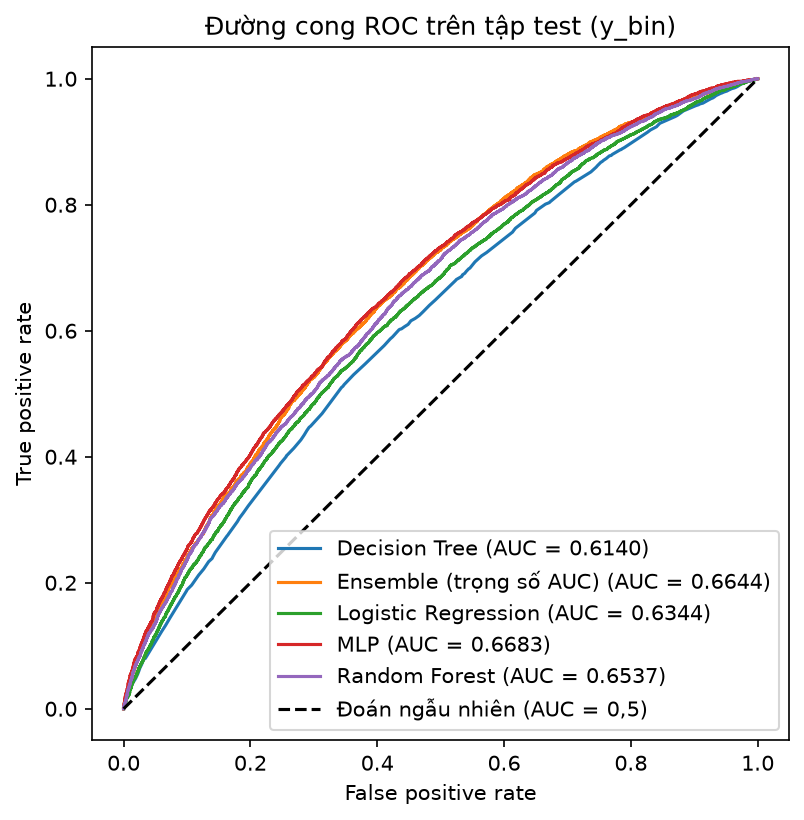
\includegraphics[width=\linewidth,keepaspectratio]{hinh/roc_curves.png}
  \caption{Đường cong ROC trên tập test}
\end{figure}

\textbf{Confusion matrix} (phần trăm theo hàng):

\begin{figure}[H]
  \centering
  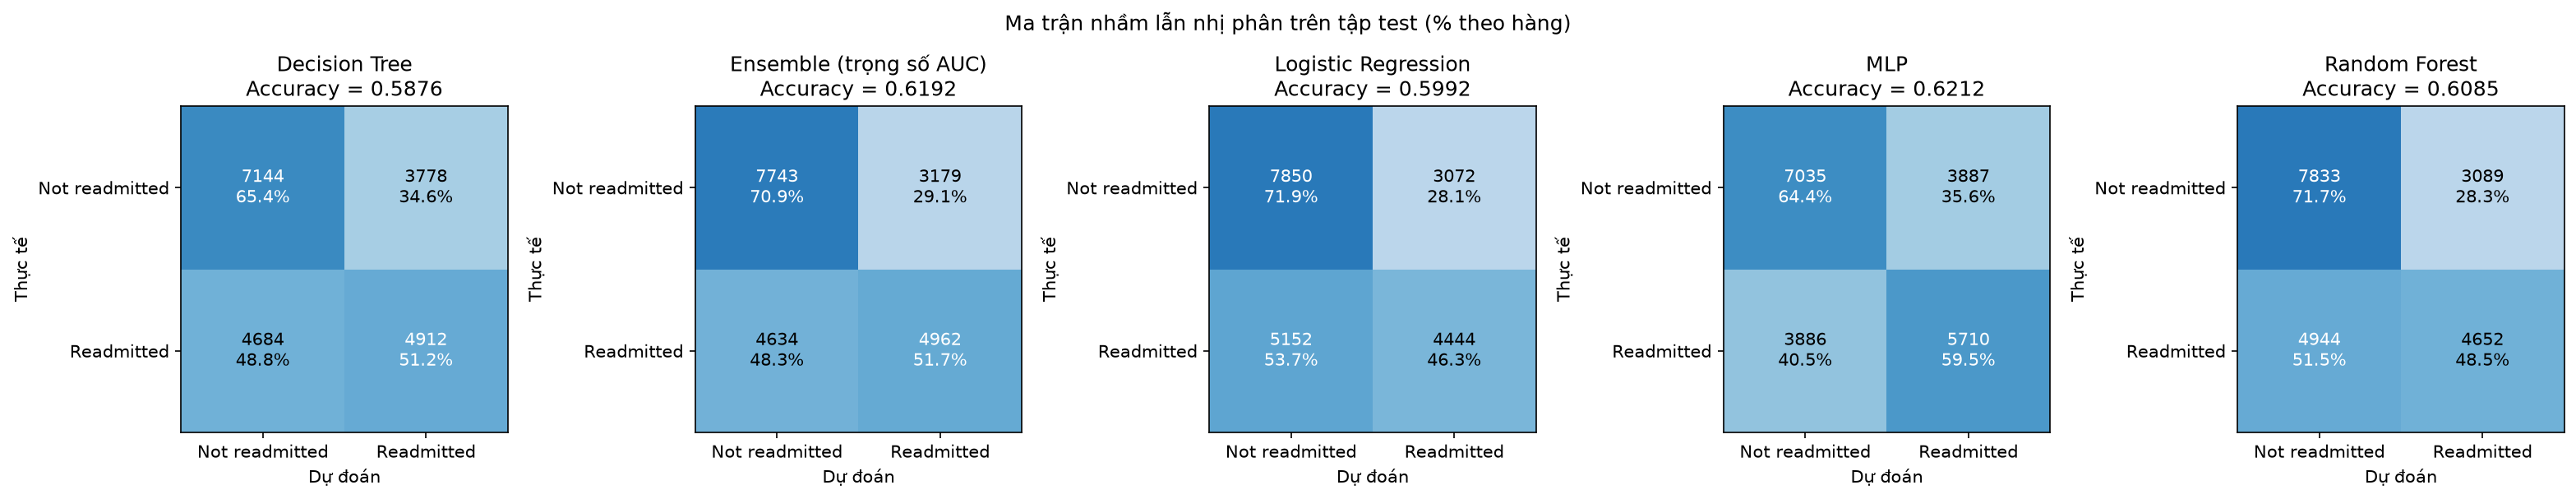
\includegraphics[width=\linewidth,keepaspectratio]{hinh/confusion_binary.png}
  \caption{Confusion matrix nhị phân}
\end{figure}

\textbf{Nhận xét.}

\begin{itemize}
  \item Cả năm mô hình đều vượt mốc đoán lớp đa số (0,5323) từ 0,055 (Decision Tree) đến 0,089 (MLP) về accuracy, và có AUC từ 0,6140 đến 0,6683, tức là phân biệt được hai lớp tốt hơn đoán ngẫu nhiên (0,5) nhưng ở mức vừa phải. Accuracy 0,59–0,62 nằm trong khoảng 0,59–0,63 mà bài báo tham khảo báo cáo.
  \item Thứ hạng theo accuracy và theo AUC trùng nhau: MLP, Ensemble, Random Forest, Logistic Regression, Decision Tree. Đường ROC của MLP và Ensemble gần như chồng khít và nằm trên các đường còn lại ở hầu hết mọi ngưỡng; Decision Tree thấp nhất.
  \item Ensemble theo weight AUC \textbf{không} vượt MLP đơn lẻ (AUC 0,6644 so với 0,6683; accuracy 0,6192 so với 0,6212), nhưng vượt cả ba thành viên còn lại. Một lý do có thể là weight theo AUC gần như đều nhau (0,24–0,26 mỗi mô hình, do AUC validation của bốn mô hình chỉ chênh nhau trong khoảng 0,05), nên MLP bị pha loãng bởi các mô hình yếu hơn.
  \item Decision Tree đơn lẻ kém nhất (AUC 0,6140) vì một cây dễ overfit, còn Random Forest gộp nhiều cây nên tăng AUC thêm 0,04 (0,6537).
  \item Về confusion matrix, MLP nhận ra được nhiều ca tái nhập viện nhất (recall 0,5950, cao hơn hẳn Decision Tree 0,5119 và Ensemble 0,5171), đổi lại sai 35,6\% ca không tái nhập viện. Random Forest và Logistic Regression thiên về dự đoán “không tái nhập viện” (recall 0,4848 và 0,4631). Chọn mô hình nào còn tùy mục tiêu: nếu bỏ sót ca tái nhập viện tốn kém hơn cảnh báo nhầm thì ưu tiên recall, tức là MLP, hoặc hạ decision threshold xuống dưới 0,5 cho các mô hình khác.
  \item Khoảng cách giữa các mô hình nhỏ (AUC chênh tối đa 0,054), cho thấy giới hạn chủ yếu nằm ở dữ liệu và ở việc PCA chỉ giữ 60 thành phần (5,55\% phương sai), không phải ở việc chọn thuật toán.
\end{itemize}

\subsection{MLP: ảnh hưởng của L2 và quá trình huấn luyện}

\begin{figure}[H]
  \centering
  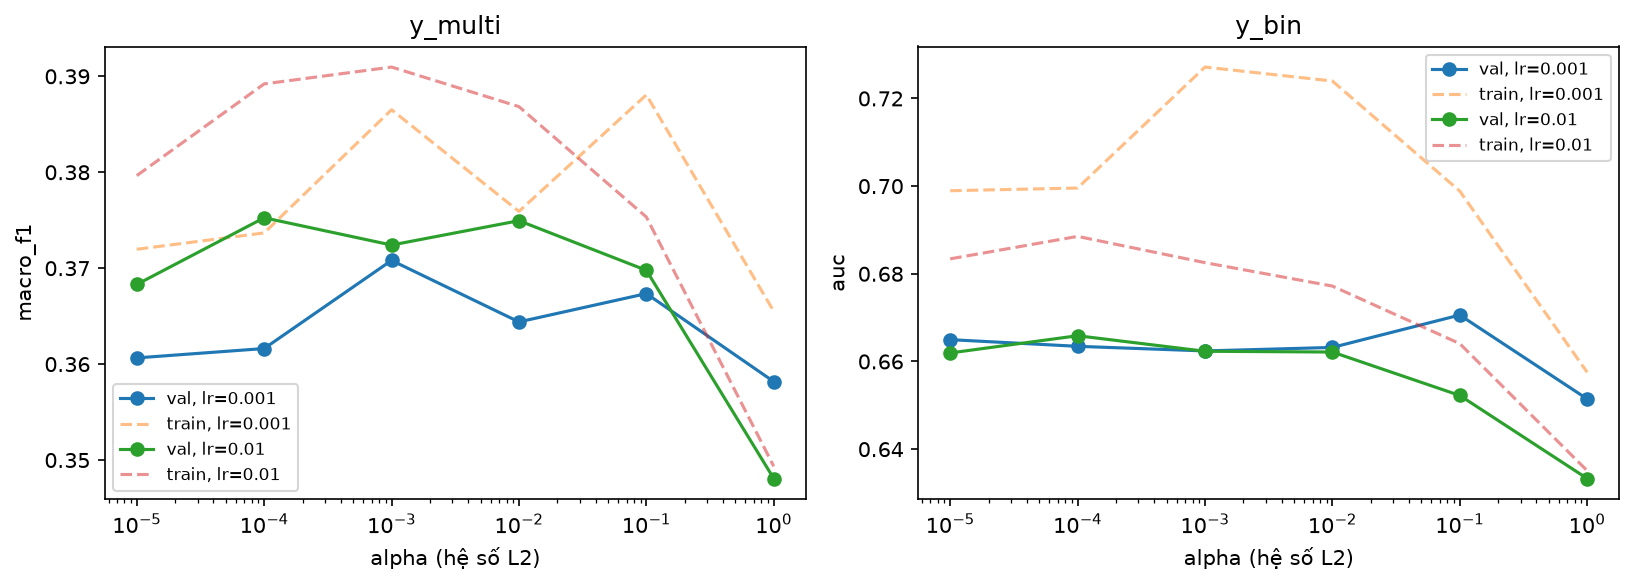
\includegraphics[width=\linewidth,keepaspectratio]{hinh/mlp_alpha_curve.png}
  \caption{Validation theo alpha}
\end{figure}

\begin{figure}[H]
  \centering
  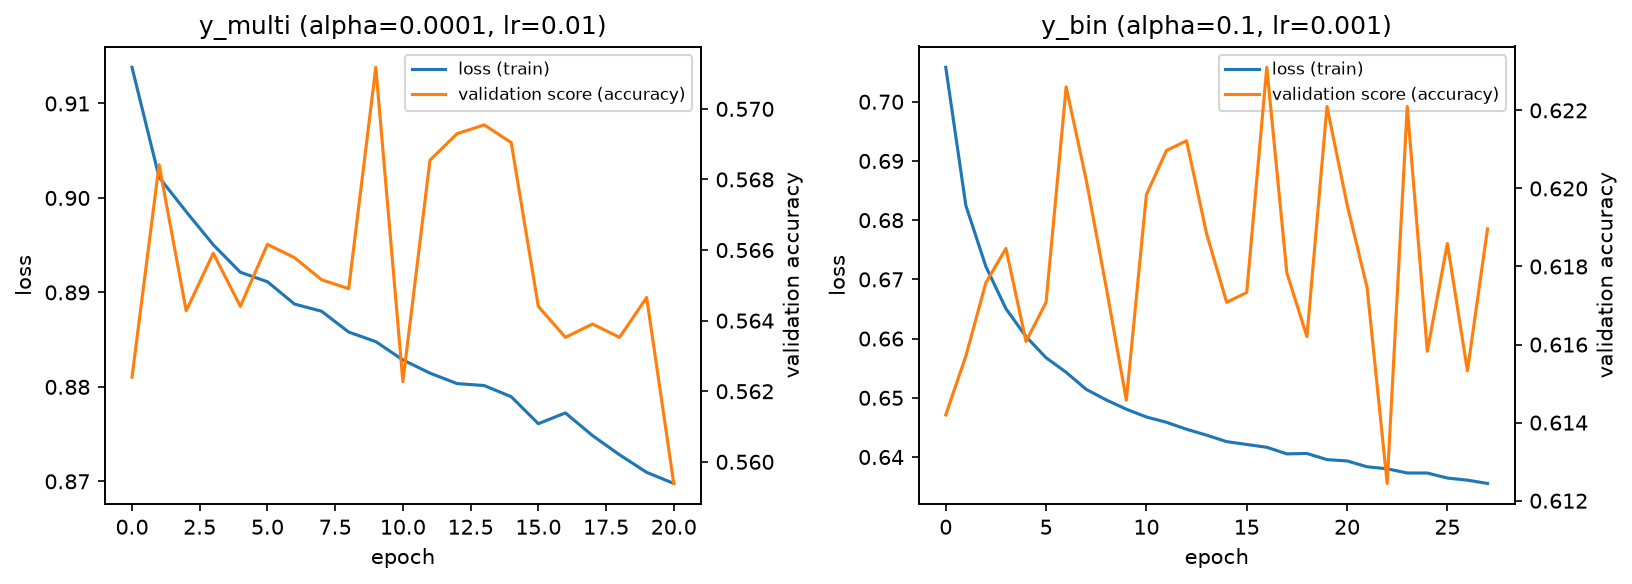
\includegraphics[width=\linewidth,keepaspectratio]{hinh/mlp_loss.png}
  \caption{Loss và validation score theo epoch}
\end{figure}

\textit{Hình: train (nét đứt) và validation theo $\alpha$, trục x log. Với \texttt{y\_\allowbreak{}bin}, train luôn cao hơn validation: chênh 0,0339 ở $\alpha = 10^{-5}$ (lr = 0,001) và 0,0283 ở $\alpha$ chọn (0,1). Chính quy hóa $L_2$ chỉ giảm nhẹ khoảng cách này; $\alpha = 1$ thì cả hai đường cùng thấp (underfit).}

\subsection{So sánh các cách đặt weight cho Ensemble}

So sánh ba cách đặt weight (ngưỡng 0,5; weight ở bảng~\ref{tb:wensemble}), kết quả ở bảng~\ref{tb:cachweight}:

{\small\setstretch{1.0}\renewcommand\arraystretch{1.1}\setlength\tabcolsep{3pt}
\begin{longtable}{|>{\raggedright\arraybackslash}p{207.49pt}|>{\centering\arraybackslash}p{33.62pt}|>{\centering\arraybackslash}p{48.68pt}|>{\centering\arraybackslash}p{33.62pt}|>{\centering\arraybackslash}p{33.62pt}|}
\caption{So sánh các cách đặt weight cho Ensemble}\label{tb:cachweight}\\
\hline
\textbf{Cách đặt weight} & \textbf{AUC} & \textbf{Accuracy} & \textbf{Recall} & \textbf{F1} \\ \hline\endfirsthead
\caption[]{So sánh các cách đặt weight cho Ensemble (tiếp theo)}\\
\hline
\textbf{Cách đặt weight} & \textbf{AUC} & \textbf{Accuracy} & \textbf{Recall} & \textbf{F1} \\ \hline\endhead
Ensemble, $w \propto$ AUC (đã dùng ở bảng~\ref{tb:nhiphan}) & 0,6644 & 0,6192 & 0,5171 & 0,5595 \\ \hline
Ensemble, trung bình đều & 0,6639 & 0,6188 & 0,5152 & 0,5584 \\ \hline
Ensemble, $w \propto$ AUC $-$ 0,5 & 0,6662 & 0,6198 & 0,5212 & 0,5618 \\ \hline
\end{longtable}
}

Ba cách chênh nhau không quá 0,0023 AUC. Cách $w \propto$ AUC $-$ 0,5 cho AUC cao nhất (0,6662) vì phân biệt các mô hình rõ hơn, nhưng vẫn thấp hơn MLP đơn lẻ (0,6683), nên kết luận ở 3.4 không đổi.

\section{ẢNH HƯỞNG CỦA CLASS IMBALANCE VÀ RANDOM FOREST TRÊN DỮ LIỆU CHƯA PCA}

Số liệu sinh từ đầu ra của bước 01–06 và kết quả Random Forest trên PCA ở 3.2.3. Môi trường: scikit-learn 1.6.1, pandas 2.2.3, numpy 2.4.6, \texttt{random\_\allowbreak{}state = 42}. Validation là 20\% train (stratified theo \texttt{y\_\allowbreak{}bin}), dùng chung với các mô hình khác; tập test chỉ dùng để báo cáo.

\subsection{Phân bố lớp}

Số mẫu và tỉ lệ từng lớp của train và test: xem bảng~\ref{tb:phanbo}.

\texttt{y\_\allowbreak{}multi} imbalanced rõ: lớp \texttt{<30} chỉ chiếm 11,47\% ở test. \texttt{y\_\allowbreak{}bin} gần cân bằng. Vì \texttt{y\_\allowbreak{}bin = 0} trùng với \texttt{y\_\allowbreak{}multi = NO}, mô hình “luôn đoán \texttt{NO}” đạt accuracy 53,23\% mà không phát hiện được ca nào, nên accuracy đơn lẻ dễ gây hiểu nhầm.

\subsection{Ảnh hưởng đến Random Forest đa lớp (\texorpdfstring{\texttt{y\_\allowbreak{}multi}}{y\textunderscore multi})}

Random Forest trên 60 PC với cấu hình tốt nhất ở 3.2.3 (50 cây, \texttt{max\_\allowbreak{}depth = None}), huấn luyện trên toàn bộ train, đánh giá trên test (bảng~\ref{tb:rfcw}):

{\footnotesize\setstretch{1.0}\renewcommand\arraystretch{1.1}\setlength\tabcolsep{3pt}
\begin{longtable}{|>{\raggedright\arraybackslash}p{99.75pt}|>{\centering\arraybackslash}p{44.54pt}|>{\centering\arraybackslash}p{47.16pt}|>{\centering\arraybackslash}p{49.44pt}|>{\centering\arraybackslash}p{49.44pt}|>{\centering\arraybackslash}p{43.75pt}|>{\centering\arraybackslash}p{74.96pt}|}
\caption{Ảnh hưởng của class weight đến Random Forest đa lớp}\label{tb:rfcw}\\
\hline
\textbf{Mô hình} & \textbf{Accuracy} & \textbf{Macro-F1} & \textbf{Recall \texttt{<30}} & \textbf{Recall \texttt{>30}} & \textbf{Recall \texttt{NO}} & \textbf{Số lần đoán \texttt{<30}} \\ \hline\endfirsthead
\caption[]{Ảnh hưởng của class weight đến Random Forest đa lớp (tiếp theo)}\\
\hline
\textbf{Mô hình} & \textbf{Accuracy} & \textbf{Macro-F1} & \textbf{Recall \texttt{<30}} & \textbf{Recall \texttt{>30}} & \textbf{Recall \texttt{NO}} & \textbf{Số lần đoán \texttt{<30}} \\ \hline\endhead
RF không class\_\allowbreak{}weight & 0,5492 & 0,3587 & 0,0076 & 0,3305 & 0,8108 & 59 / 2.353 \\ \hline
RF class\_\allowbreak{}weight=balanced & 0,5502 & 0,3542 & 0,0089 & 0,2993 & 0,8331 & 59 / 2.353 \\ \hline
Mốc: luôn đoán NO & 0,5323 & 0,2316 & 0,0000 & 0,0000 & 1,0000 & 0 / 2.353 \\ \hline
\end{longtable}
}

\textbf{Nhận xét.} RF hơn mốc “luôn đoán \texttt{NO}” 1,69 điểm phần trăm accuracy, nhưng chỉ phát hiện 0,76\% ca \texttt{<30} (đoán \texttt{<30} 59 lần trên 2.353 mẫu thật). Phần lớn macro-F1 đến từ lớp \texttt{>30} và \texttt{NO}. Dùng \texttt{class\_\allowbreak{}weight="balanced"} hầu như không cải thiện: recall \texttt{<30} chỉ đổi từ 0,0076 sang 0,0089, số lần đoán \texttt{<30} vẫn là 59, và macro-F1 còn thấp hơn (0,3542 so với 0,3587). Với cấu hình cây sâu (\texttt{max\_\allowbreak{}depth = None}), mỗi cây khớp gần hết dữ liệu train nên có thể class weight ít tác động đến dự đoán (giả thuyết này chưa được kiểm chứng riêng). Hạn chế của thí nghiệm: chỉ thử một cấu hình RF và một cách cân bằng, chưa thử lấy mẫu lại (oversampling/undersampling) hay giảm \texttt{max\_\allowbreak{}depth} khi dùng weight.

Kết nối với k-NN và Softmax (mục 3.3): Softmax đoán \texttt{<30} rất ít lần và accuracy chỉ hơn mốc \texttt{NO} vài điểm phần trăm, cùng triệu chứng như RF: mô hình tối ưu cho lớp đa số.

\subsection{Ngưỡng quyết định nhị phân (\texorpdfstring{\texttt{y\_\allowbreak{}bin}}{y\textunderscore bin})}

Dùng xác suất của RF PCA (400 cây, \texttt{max\_\allowbreak{}depth = 20}), chọn ngưỡng trên validation để tối đa F1 của lớp 1 thay vì 0,5; AUC không đổi vì chỉ đổi ngưỡng (bảng~\ref{tb:nguong}):

{\footnotesize\setstretch{1.0}\renewcommand\arraystretch{1.1}\setlength\tabcolsep{3pt}
\begin{longtable}{|>{\raggedright\arraybackslash}p{168.40pt}|>{\centering\arraybackslash}p{44.54pt}|>{\centering\arraybackslash}p{43.62pt}|>{\centering\arraybackslash}p{30.79pt}|>{\centering\arraybackslash}p{30.79pt}|>{\centering\arraybackslash}p{30.79pt}|}
\caption{Ảnh hưởng của ngưỡng quyết định đến Random Forest nhị phân}\label{tb:nguong}\\
\hline
\textbf{Ngưỡng} & \textbf{Accuracy} & \textbf{Precision} & \textbf{Recall} & \textbf{F1} & \textbf{AUC} \\ \hline\endfirsthead
\caption[]{Ảnh hưởng của ngưỡng quyết định đến Random Forest nhị phân (tiếp theo)}\\
\hline
\textbf{Ngưỡng} & \textbf{Accuracy} & \textbf{Precision} & \textbf{Recall} & \textbf{F1} & \textbf{AUC} \\ \hline\endhead
Ngưỡng 0,5 (t = 0,50) & 0,6085 & 0,6010 & 0,4848 & 0,5367 & 0,6537 \\ \hline
Ngưỡng chọn trên validation (t = 0,32) & 0,5277 & 0,4974 & 0,9408 & 0,6507 & 0,6537 \\ \hline
\end{longtable}
}

\textbf{Nhận xét.} Ngưỡng chọn trên validation là 0,32. Recall tăng từ 0,4848 lên 0,9408 và F1 từ 0,5367 lên 0,6507, nhưng accuracy giảm từ 0,6085 xuống 0,5277 và precision từ 0,6010 xuống 0,4974. Ở ngưỡng thấp như vậy mô hình gần như dự đoán “tái nhập viện” cho hầu hết bệnh nhân, nên F1 tăng chủ yếu vì lớp 1 chiếm gần một nửa dữ liệu chứ không vì mô hình phân biệt tốt hơn (AUC vẫn là 0,6537). Chọn ngưỡng nên dựa vào chi phí thực tế của bỏ sót ca so với cảnh báo nhầm, không chỉ F1.

\subsection{Random Forest trên One-Hot (chưa PCA)}

RF 200 cây trên ma trận thưa 2.396 cột One-Hot (bước 04), \texttt{max\_\allowbreak{}features = "sqrt"}; \texttt{max\_\allowbreak{}depth} chọn trên validation trong \{8, 12, 16, 20, \texttt{None}\} (AUC validation lần lượt 0,6780, 0,6823, 0,6853, 0,6875 và 0,6915: tăng đơn điệu theo độ sâu, cao nhất ở \texttt{None}; các giá trị này in ra khi chạy script, không lưu thành csv) (bảng~\ref{tb:rfraw}):

{\footnotesize\setstretch{1.0}\renewcommand\arraystretch{1.1}\setlength\tabcolsep{3pt}
\begin{longtable}{|>{\raggedright\arraybackslash}p{92.94pt}|>{\centering\arraybackslash}p{30.30pt}|>{\raggedright\arraybackslash}p{52.19pt}|>{\centering\arraybackslash}p{72.56pt}|>{\centering\arraybackslash}p{66.18pt}|>{\centering\arraybackslash}p{45.41pt}|}
\caption{Random Forest trên One-Hot và trên PCA (bài toán nhị phân)}\label{tb:rfraw}\\
\hline
\textbf{Dữ liệu} & \textbf{Số cây} & \textbf{\texttt{max\_\allowbreak{}depth}} & \textbf{AUC validation} & \textbf{Test Accuracy} & \textbf{Test AUC} \\ \hline\endfirsthead
\caption[]{Random Forest trên One-Hot và trên PCA (bài toán nhị phân) (tiếp theo)}\\
\hline
\textbf{Dữ liệu} & \textbf{Số cây} & \textbf{\texttt{max\_\allowbreak{}depth}} & \textbf{AUC validation} & \textbf{Test Accuracy} & \textbf{Test AUC} \\ \hline\endhead
One-Hot (chưa PCA) & 200 & None & 0,6915 & 0,6413 & 0,6957 \\ \hline
PCA 60 chiều (3.2.3) & 400 & 20 & 0,6542 & 0,6085 & 0,6537 \\ \hline
\end{longtable}
}

\textbf{Nhận xét.} RF trên One-Hot tốt hơn RF trên PCA 0,0420 AUC và 3,28 điểm phần trăm accuracy: PCA 60 thành phần chỉ giữ khoảng 5,55\% tổng phương sai nên mất thông tin dự báo. Hai cấu hình không hoàn toàn so sánh được (200 cây với \texttt{max\_\allowbreak{}depth = None} so với 400 cây với \texttt{max\_\allowbreak{}depth = 20}, lưới và phương pháp chọn khác nhau), nhưng khoảng cách 0,0420 đủ lớn để kết luận xu hướng.

\subsection{Feature importance}

\begin{sidewaysfigure}[p]% trang xoay ngang
  \centering
  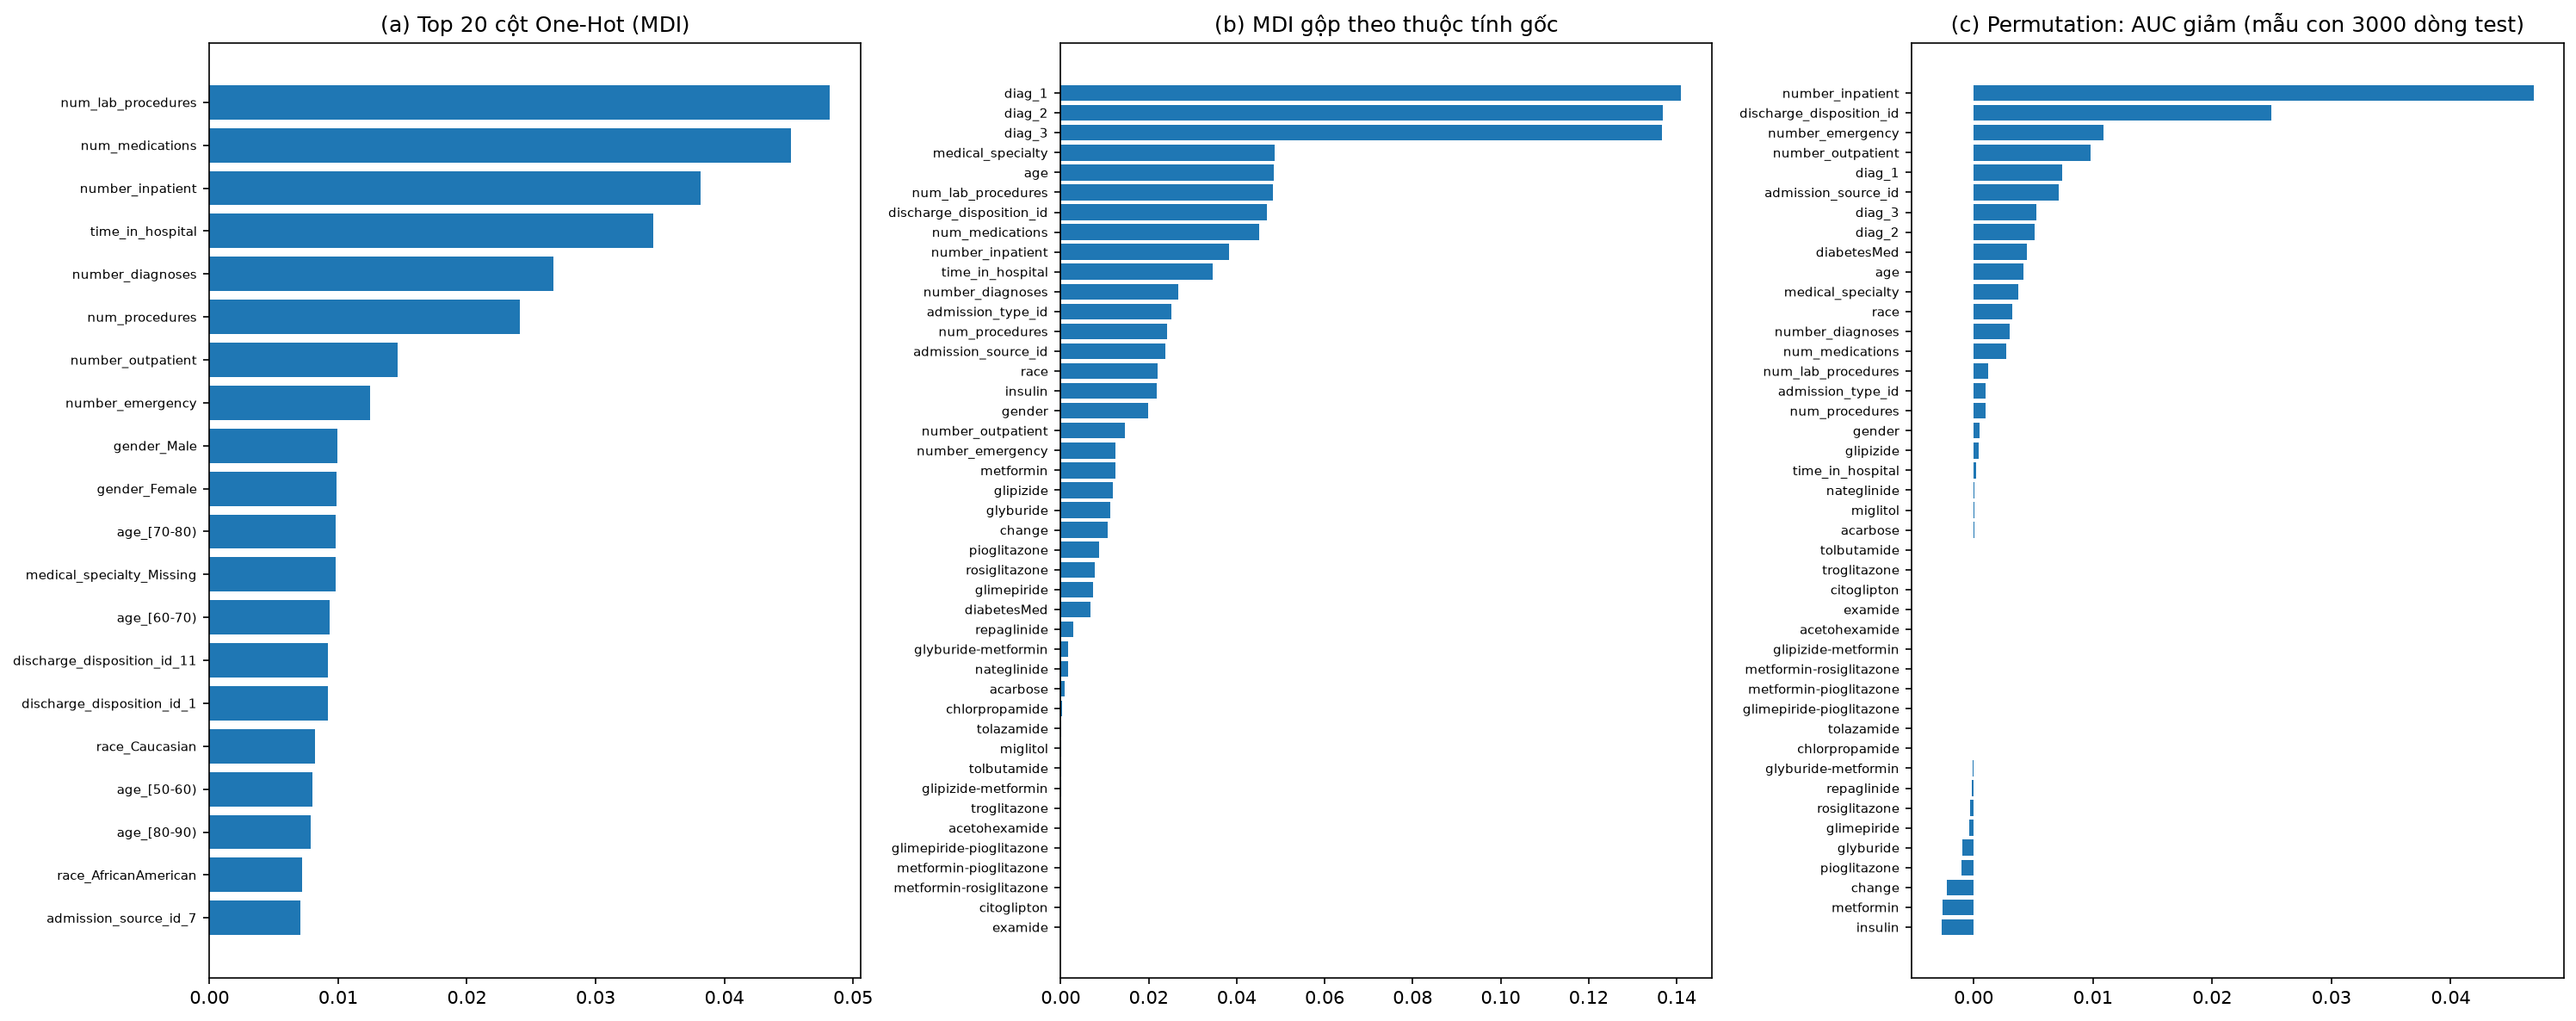
\includegraphics[width=\linewidth,height=0.78\textwidth,keepaspectratio]{hinh/rf_raw_importance.png}
  \caption{Feature importance}\label{fig:landscape}
\end{sidewaysfigure}

\textit{Hình: (a) top 20 cột One-Hot theo MDI (Mean Decrease in Impurity, độ giảm độ không thuần khiết trung bình); (b) MDI gộp theo thuộc tính gốc; (c) permutation importance theo thuộc tính gốc (AUC giảm khi hoán vị cả nhóm cột, trên mẫu 3.000 dòng test, trung bình 3 lần).}

Top 10 theo MDI (tổng độ giảm Gini, đã cộng các cột cùng thuộc tính gốc) và theo permutation importance (bảng~\ref{tb:top10}):

{\small\setstretch{1.0}\renewcommand\arraystretch{1.1}\setlength\tabcolsep{3pt}
\begin{longtable}{|>{\centering\arraybackslash}p{28.69pt}|>{\raggedright\arraybackslash}p{147.62pt}|>{\centering\arraybackslash}p{37.57pt}|>{\raggedright\arraybackslash}p{147.62pt}|>{\centering\arraybackslash}p{53.93pt}|}
\caption{Top 10 thuộc tính theo MDI và theo permutation importance}\label{tb:top10}\\
\hline
\textbf{Hạng} & \textbf{Thuộc tính (MDI)} & \textbf{MDI} & \textbf{Thuộc tính (permutation)} & \textbf{AUC giảm} \\ \hline\endfirsthead
\caption[]{Top 10 thuộc tính theo MDI và theo permutation importance (tiếp theo)}\\
\hline
\textbf{Hạng} & \textbf{Thuộc tính (MDI)} & \textbf{MDI} & \textbf{Thuộc tính (permutation)} & \textbf{AUC giảm} \\ \hline\endhead
1 & \texttt{diag\_\allowbreak{}1} & 14,11\% & \texttt{number\_\allowbreak{}inpatient} & 0,0470 \\ \hline
2 & \texttt{diag\_\allowbreak{}2} & 13,69\% & \texttt{discharge\_\allowbreak{}disposition\_\allowbreak{}id} & 0,0250 \\ \hline
3 & \texttt{diag\_\allowbreak{}3} & 13,67\% & \texttt{number\_\allowbreak{}emergency} & 0,0109 \\ \hline
4 & \texttt{medical\_\allowbreak{}specialty} & 4,86\% & \texttt{number\_\allowbreak{}outpatient} & 0,0098 \\ \hline
5 & \texttt{age} & 4,85\% & \texttt{diag\_\allowbreak{}1} & 0,0074 \\ \hline
6 & \texttt{num\_\allowbreak{}lab\_\allowbreak{}procedures} & 4,82\% & \texttt{admission\_\allowbreak{}source\_\allowbreak{}id} & 0,0071 \\ \hline
7 & \texttt{discharge\_\allowbreak{}disposition\_\allowbreak{}id} & 4,69\% & \texttt{diag\_\allowbreak{}3} & 0,0053 \\ \hline
8 & \texttt{num\_\allowbreak{}medications} & 4,52\% & \texttt{diag\_\allowbreak{}2} & 0,0051 \\ \hline
9 & \texttt{number\_\allowbreak{}inpatient} & 3,82\% & \texttt{diabetesMed} & 0,0045 \\ \hline
10 & \texttt{time\_\allowbreak{}in\_\allowbreak{}hospital} & 3,45\% & \texttt{age} & 0,0042 \\ \hline
\end{longtable}
}

\textbf{Nhận xét.} Theo MDI, ba mã chẩn đoán \texttt{diag\_\allowbreak{}1}, \texttt{diag\_\allowbreak{}2}, \texttt{diag\_\allowbreak{}3} chiếm tổng 41,5\% feature importance và đứng đầu. Nhưng MDI thiên vị các thuộc tính có nhiều giá trị: mỗi mã chẩn đoán được One-Hot thành hàng trăm cột, mỗi cột có nhiều cơ hội được chọn để chia nút. Permutation importance (đo trực tiếp mức giảm AUC khi phá thuộc tính) cho bức tranh khác: \textbf{\texttt{number\_\allowbreak{}inpatient}} là quan trọng nhất (AUC giảm 0,0470), tiếp theo là \texttt{discharge\_\allowbreak{}disposition\_\allowbreak{}id} (0,0250), còn \texttt{diag\_\allowbreak{}1} chỉ giảm 0,0074. Điều này khớp với trực giác lâm sàng: số lần nhập viện nội trú trước đó và cách xuất viện liên quan trực tiếp đến nguy cơ tái nhập viện. Permutation chạy trên 3.000 dòng với 3 lần lặp nên các giá trị nhỏ (dưới 0,005) có nhiễu và không nên xếp hạng chặt.

Khác với các thành phần PCA (mỗi thành phần là tổ hợp tuyến tính của hàng nghìn cột One-Hot nên không đọc được ý nghĩa), RF trên One-Hot cho phép chỉ ra từng thuộc tính gốc đóng góp bao nhiêu. Đây là lợi thế diễn giải của việc bỏ PCA, ngoài chênh lệch về hiệu quả dự báo ở mục 3.5.4.


% ======================================================================
\chuong{Kết luận}
\section{KẾT LUẬN}

\subsection{Tổng kết}

Báo cáo xây dựng quy trình dự đoán tái nhập viện của bệnh nhân đái tháo đường trên bộ dữ liệu 130 bệnh viện Hoa Kỳ (101.766 lượt nhập viện). Sau khi bỏ thuộc tính định danh, cột khuyết trên 50\% và 1.522 dòng khuyết chẩn đoán, còn 100.244 dòng, chia 79.726 train và 20.518 test theo bệnh nhân để tránh data leakage. Dữ liệu được mã hóa One-Hot (2.396 cột) rồi giảm còn 60 thành phần bằng PCA. Các mô hình k-NN, Softmax Regression, Decision Tree, Random Forest, MLP và Ensemble theo weight AUC được so sánh trên cả nhãn đa lớp và nhãn nhị phân.

\subsection{Kết quả chính}

\begin{itemize}
  \item \textbf{Bài toán đa lớp:} accuracy cao không đồng nghĩa với mô hình tốt. Softmax đã scale đạt accuracy cao nhất (0,5505) nhưng gần như không phát hiện lớp \texttt{<30} (recall 0,0\%); k-NN chưa scale có macro-F1 cao nhất (0,3807) và F1 lớp \texttt{<30} cao nhất (0,1327). Mốc ``luôn đoán \texttt{NO}'' đạt accuracy 0,5323.
  \item \textbf{Bài toán nhị phân:} cả năm mô hình đều vượt mốc đoán lớp đa số, với AUC từ 0,6140 đến 0,6683. MLP tốt nhất (accuracy 0,6212, AUC 0,6683); Ensemble theo weight AUC (AUC 0,6644) không vượt MLP đơn lẻ nhưng vượt Random Forest, Logistic Regression và Decision Tree.
  \item \textbf{Ảnh hưởng của PCA:} 60 thành phần chỉ giữ khoảng 5,55\% phương sai. Random Forest trên One-Hot (chưa PCA) đạt AUC 0,6957, cao hơn Random Forest trên PCA (0,6537) khoảng 0,042.
  \item \textbf{Yếu tố liên quan:} theo permutation importance, \texttt{number\_\allowbreak{}inpatient} và \texttt{discharge\_\allowbreak{}disposition\_\allowbreak{}id} là hai thuộc tính quan trọng nhất; ba mã chẩn đoán đứng đầu theo MDI nhưng bị đánh giá cao do có nhiều giá trị khác nhau.
\end{itemize}

\subsection{Hạn chế và hướng phát triển}

Giới hạn chủ yếu nằm ở dữ liệu và bước giảm chiều: khoảng cách giữa các mô hình nhỏ (AUC chênh tối đa 0,054) và lớp \texttt{<30} (11\%) gần như chưa được nhận diện. Các hướng cải thiện gồm: huấn luyện trực tiếp trên ma trận One-Hot thưa hoặc dùng nhiều thành phần PCA hơn; dùng class weight hoặc lấy mẫu lại cho lớp \texttt{<30}; chọn decision threshold theo chi phí bỏ sót ca so với cảnh báo nhầm; và thử các mô hình boosting. Ngoài ra, mỗi cấu hình chỉ chạy với một \texttt{random\_\allowbreak{}state}, nên chênh lệch nhỏ giữa các mô hình cần được kiểm tra thêm bằng nhiều lần chia dữ liệu.


% ======================================================================
\phansau
\phantomsection\addcontentsline{toc}{chapter}{\mdseries Tài liệu tham khảo}
% Mục 6.7: đánh số theo thứ tự trích dẫn; tên tác giả đậm; tên tạp chí viết đầy đủ.
\begin{thebibliography}{99}
\bibitem{tl1} \textbf{J. J. Khanam, S. Y. Foo} – A comparison of machine learning algorithms for diabetes prediction, ICT Express \textbf{7(4)} (2021) 432–439.
\bibitem{tl2} \textbf{Md. Maniruzzaman et al.} – Accurate diabetes risk stratification using machine learning: Role of missing value and outliers, Journal of Medical Systems \textbf{42(5)} (2018) 92.
\bibitem{tl3} \textbf{T. S. Brisimi et al.} – Predicting diabetes-related hospitalizations based on electronic health records, Statistical Methods in Medical Research \textbf{28(12)} (2019) 3667–3682.
\bibitem{tl4} \textbf{D. Dutta, D. Paul, P. Ghosh} – Analysing feature importances for diabetes prediction using machine learning, IEEE IEMCON (2018) 924–928.
\bibitem{tl5} \textbf{D. Sisodia, D. S. Sisodia} – Prediction of diabetes using classification algorithms, Procedia Computer Science \textbf{132} (2018) 1578–1585.
\bibitem{tl6} \textbf{Md. K. Hasan et al.} – Diabetes prediction using ensembling of different machine learning classifiers, IEEE Access \textbf{8} (2020) 76516–76531.
\bibitem{tl7} \textbf{B. Strack et al.} – Impact of HbA1c measurement on hospital readmission rates: Analysis of 70,000 clinical database patient records, BioMed Research International (2014) 781670.
\bibitem{tl8} \textbf{D. Wang} – Predicting diabetes health outcomes using a variety of models. Stanford CS229 project report.
\end{thebibliography}


\phuluc
\chapter*{Phụ lục. Mã nguồn và cấu trúc kết quả}
\addcontentsline{toc}{chapter}{\mdseries Phụ lục. Mã nguồn và cấu trúc kết quả}

Mã nguồn của toàn bộ thực nghiệm: \url{https://github.com/chiensondung/HCMUT-AnIntroductiontoMachineLearningandApplication-Project}. Mỗi bước là một script trong thư mục \texttt{src/\allowbreak{}}, đọc kết quả của bước trước từ thư mục \texttt{output/\allowbreak{}} và ghi kết quả của mình vào đó. Các hình minh họa trong báo cáo do các script này sinh ra, tên file ảnh ghi ở cột bên phải của bảng~\ref{tb:scripts}.

{\small\setstretch{1.0}\renewcommand\arraystretch{1.1}\setlength\tabcolsep{3pt}
\begin{longtable}{|>{\centering\arraybackslash}p{27.26pt}|>{\raggedright\arraybackslash}p{203.69pt}|>{\raggedright\arraybackslash}p{203.69pt}|}
\caption{Các script và file kết quả chính}\label{tb:scripts}\\
\hline
\textbf{Bước} & \textbf{Script (\texttt{src/\allowbreak{}})} & \textbf{File kết quả chính (\texttt{output/\allowbreak{}})} \\ \hline\endfirsthead
\caption[]{Các script và file kết quả chính (tiếp theo)}\\
\hline
\textbf{Bước} & \textbf{Script (\texttt{src/\allowbreak{}})} & \textbf{File kết quả chính (\texttt{output/\allowbreak{}})} \\ \hline\endhead
01 & \texttt{01\_\allowbreak{}explore\_\allowbreak{}and\_\allowbreak{}drop\_\allowbreak{}ids.py} & \texttt{step1.csv} \\ \hline
02 & \texttt{02\_\allowbreak{}missing\_\allowbreak{}stats\_\allowbreak{}and\_\allowbreak{}filter.py} & \texttt{missing\_\allowbreak{}rate.csv}, \texttt{step2.csv} \\ \hline
03 & \texttt{03\_\allowbreak{}data\_\allowbreak{}preprocessing\_\allowbreak{}splitting.py} & \texttt{train.csv}, \texttt{test.csv} \\ \hline
04 & \texttt{04\_\allowbreak{}one\_\allowbreak{}hot\_\allowbreak{}encoding.py} & \texttt{X\_\allowbreak{}\{train,test\}\_\allowbreak{}onehot.npz}, \texttt{y\_\allowbreak{}\{train,test\}.csv}, \texttt{onehot\_\allowbreak{}columns.txt} \\ \hline
05 & \texttt{05\_\allowbreak{}pca.py} & \texttt{X\_\allowbreak{}\{train,test\}\_\allowbreak{}pca.npy}, \texttt{pca\_\allowbreak{}summary.csv} \\ \hline
06 & \texttt{06\_\allowbreak{}feature\_\allowbreak{}scaling\_\allowbreak{}pca\_\allowbreak{}analysis.py} & \texttt{X\_\allowbreak{}\{train,test\}\_\allowbreak{}pca\_\allowbreak{}scaled.npy}, \texttt{eigenvalues.csv}, \texttt{top5\_\allowbreak{}pc\_\allowbreak{}dac\_\allowbreak{}trung.csv} \\ \hline
07a & \texttt{07a\_\allowbreak{}knn.py} & \texttt{knn\_\allowbreak{}results.csv}, \texttt{knn\_\allowbreak{}k\_\allowbreak{}curve.png} \\ \hline
07b & \texttt{07b\_\allowbreak{}softmax\_\allowbreak{}regression.py} & \texttt{softmax\_\allowbreak{}results.csv}, \texttt{softmax\_\allowbreak{}loss.png} \\ \hline
08a & \texttt{08a\_\allowbreak{}decision\_\allowbreak{}tree.py} & \texttt{dt\_\allowbreak{}results.csv}, \texttt{dt\_\allowbreak{}depth\_\allowbreak{}curve.png} \\ \hline
08b & \texttt{08b\_\allowbreak{}random\_\allowbreak{}forest.py} & \texttt{rf\_\allowbreak{}results.csv}, \texttt{rf\_\allowbreak{}depth\_\allowbreak{}curve.png} \\ \hline
09a & \texttt{09a\_\allowbreak{}mlp.py} & \texttt{mlp\_\allowbreak{}results.csv}, \texttt{mlp\_\allowbreak{}alpha\_\allowbreak{}curve.png}, \texttt{mlp\_\allowbreak{}loss.png} \\ \hline
09b & \texttt{09b\_\allowbreak{}ensemble.py} & \texttt{ensemble\_\allowbreak{}weights.csv}, \texttt{ensemble\_\allowbreak{}results.csv} \\ \hline
10 & \texttt{10\_\allowbreak{}evaluation.py} & \texttt{accuracy\_\allowbreak{}summary.csv}, \texttt{confusion\_\allowbreak{}matrices.png} \\ \hline
11 & \texttt{11\_\allowbreak{}binary\_\allowbreak{}evaluation.py} & \texttt{binary\_\allowbreak{}summary.csv}, \texttt{roc\_\allowbreak{}curves.png}, \texttt{confusion\_\allowbreak{}binary.png} \\ \hline
12 & \texttt{12\_\allowbreak{}imbalance\_\allowbreak{}and\_\allowbreak{}rf\_\allowbreak{}raw.py} & \texttt{imbalance\_\allowbreak{}*.csv}, \texttt{rf\_\allowbreak{}raw\_\allowbreak{}*.csv}, \texttt{rf\_\allowbreak{}raw\_\allowbreak{}importance.png} \\ \hline
\end{longtable}
}

% \taobiasau% Bìa 3 + Bìa 4 (trống)
\end{document}